%Hauptdokument der Erstsemesterzeitschrift "Erste" der Fachgruppe Informatik
\documentclass[]{papertex}

\usepackage[utf8]{inputenc}
\usepackage{geometry}
\usepackage{graphicx}
\usepackage{amssymb}
%\usepackage[T1]{fontenc}
\usepackage{multicol}
\usepackage{comment}
\usepackage[ngerman]{babel}
\usepackage{wrapfig}
\usepackage[babel,german=quotes]{csquotes}
\usepackage[obeyFinal]{todonotes}
\usepackage{etoolbox}
\usepackage{sectsty}
\usepackage[hidelinks]{hyperref}
\usepackage{tabularx}
\usepackage{pdfpages}

\renewcommand{\familydefault}{\sfdefault}

%\clubpenalty = 10000
%\widowpenalty = 10000 
%\displaywidowpenalty = 10000

% Trennregeln
\hyphenation{
	AStA
	Mit-be-wohnerIn-nen
	Pro-fessorInnen
	erwischt
	viiieel
	y-Nummer
	Uniaccount
}

% left aligned sections
%\allsectionsfont{\raggedright}


\settoggle{winter}{true}
\setcounter{version}{6}


% Toggles between winter term and summer term 
\newtoggle{winter}

% This system is meant to make updating the Erste for the new semster simple. Every semster gets a new version number that is larger than the previous one (assigned in 1-te.tex). 
% By using \tocheck, defined below, todos can be left in the source and disabled one by one by incresing the version number of the tocheck. Once all todos are adressed, the new version can be released. Later all todos can be enabled again by incrementing the version number.
\newcounter{version}

% Defines a conditional todo. 2 mandatory arguments:
% 1st param, Valid to version: This todo has been adressd as of the given version
% 2nd param, Todo description: What needs to be done to adress this todo
\newrobustcmd{\tocheck}[2]{
	\ifnumless{#1}{\value{version}}{
		\todo[inline]{#2}
	}{}
}

% Versioned url. 2 mandatory arguments:
% 1st param, Valid to version: This url is still valid as of version
% 2nd param, URL: The url
\newrobustcmd{\verUrl}[2]{\ifnumless{#1}{\value{version}}{\todo[inline]{Check \url{#2}}}{}\url{#2}}
\newrobustcmd{\verHref}[4][]{\ifnumless{#2}{\value{version}}{\todo[inline]{Check \url{#3}}}{}\href[#1]{#3}{\nolinkurl{#4}}}

\newrobustcmd{\fginfoUrl}[0]{\verUrl{4}{http://fginfo.cs.tu-bs.de}}

%%

\newrobustcmd{\xkcd}[2]{
	\begin{center}
		\includegraphics[#1]{bilder/XKCD/#2}
	\end{center}
}

\settoggle{winter}{false}
\setcounter{version}{3}

\begin{document}
	\thispagestyle{empty}
	\clearpage

	\listoftodos
	\clearpage

	\setcounter{page}{1}
	\tableofcontents
	% !TEX root = ../1-te.tex

\section{Vorwort}
\label{vorwort}
	\begin{multicols}{2}
	\subsection*{Willkommen in der Informatik!}	

	Das neue Semester an der TU Braunschweig beginnt und du bist dabei. Die Fachgruppe Informatik (s. Seite \pageref{fachgruppe}) begrüßt dich ganz herzlich an der Uni und möchte dir mit der \enquote{1-ten} den Start vereinfachen. Diese Erstsemesterzeitung der Informatiker soll dir dabei helfen, Antworten auf viele Fragen, die sich zu Beginn des Studiums stellen, zu beantworten.

	\subsubsection*{Aufbau dieses Heftes}
		Der Fokus der ersten Seiten liegt auf den vielen Fragen zum Studienbeginn, deinem Studiengang und der Infrastruktur der Uni. Wir erklären, wie Studienplanung funktioniert und was für Bachelor und Master wichtig ist.
Der Fachgruppenrat Informatik stellt sich vor und beantwortet die Fragen, wer er ist und was er macht.


	\columnbreak

	\begin{center}
		
\includegraphics[width=.7\columnwidth]{bilder/fg-logo/fg-logo.pdf}
	\end{center}

	\subsubsection*{Der Blog}
		Der Fachgruppenrat Informatik betreibt den Blog FGInfo (\fginfoUrl). Dort werden unsere Termine und Veranstaltungen, z.B. Spieleabende, angekündigt und über die hochschulpolitische Arbeit berichtet.
Zusätzlich pflegt die Fachgruppe ein Wiki mit vielen Infos, Tipps und Wissenswertes rund um die Informatik-Studiengänge.
Dieses Heft, die 1-te, gibt es dort auch noch einmal zu finden. Mitunter
ergeben sich noch nach dem Druck Änderungen, gerade bei Terminen, also schau auf jeden Fall dort rein!

	\vspace*{0.5cm}

	Viel Spaß und Erfolg im  Studium wünscht  die\\
	\hspace*{2cm}Fachgruppe Informatik

	\end{multicols}

	\newpage

	\section{Die ersten Tage}
		% !TEX root = ../../1-te.tex

\subsection{Checkliste}
\label{checkliste}
	Hier wird zusammengefasst, was du in den ersten Tagen des Studiums unbedingt erledigen solltest. Wenn du die ToDos auf der Checkliste nach Erledigung abhakst, verlierst du nicht den Überblick und vergisst nichts.
	
\vspace*{0.5cm}
% !TEX root = ../../1-te.tex

\begin{tabular}{|p{3mm}|l|l|c|c|}
\hline \checkmark 
       & \textbf{Todo}             & \textbf{Zu erledigen bis}                                  & \textbf{Seite}               & \textbf{Muss?} \\ 
\hline & BAföG beantragen          & Spätestens Ende \iftoggle{winter}{Oktober}{April}          & \pageref{todobafoeg}         & optional \\ 
\hline & Wohnsitz Ummelden         & 1 Woche nach Umzug                                         & \pageref{todoummelden}       & ja \\ 
\hline & Mailinglisten             & So früh wie möglich                                        & \pageref{mailinglisten}      & ja \\ 
\hline & Studiengrobplanung        & Vor dem Stundenplanbauen                                   & \pageref{grob}               & ja \\ 
\hline & Auflagen klären           & So früh wie möglich, final: Ende 2. Semester               & \pageref{auflagen}           & nur Master \\ 
\hline & Persönlicher Stundenplan  & Siehe Terminzettel der Fachgruppe                          & \pageref{masterstundenplan}  & ja \\ 
\hline & Prüfungsbogen             & Apätestens \iftoggle{winter}{Dezember}{Mai}                & \pageref{todoanmeldung}      & ja \\ 
\hline & Prüfungsanmeldung         & Anmeldewoche (30.05 - 03.06) oder Online (09.05 - 20.06)   & \pageref{todoanmeldung}      & ja \\ 
\hline & Blog abonnieren           & So früh wie möglich                                        & \pageref{fachgruppe}         & ja \\ 
\hline & Prüfungsordnung lesen     & Zu den ersten Klausuren                                    & \pageref{po}                 & ja \\ 
\hline & TUcard validieren         & Zu Beginn und zu jedem neuen Semester                      & \pageref{tucard}             & ja \\
\hline & Bibliotheksausweis        & Vor der ersten Buchausleihe                                & \pageref{todobib}            & optional \\
\hline & Kopierkarte               & Wenn man was kopieren muss                                 & \pageref{todobib}            & optional \\ 
\hline
\end{tabular} 
\tocheck{2}{Exakte Daten Anmeldewoche einfügen, s.\url{https://www.tu-braunschweig.de/fk1/service/informatik/pa/}}

\begin{multicols}{2}

\subsubsection{BAföG}
	\label{todobafoeg}

	Wer BAföG beantragen möchte, sollte sich am besten gründlich informieren. Sehr zu empfehlen ist da: \\
	\verUrl{2}{http://www.bafoeg.bmbf.de/}
 
	Förderungsanträge gibt es zum Download oder in Papierform im EG des BAföG-Amtes, Wilhelmstraße 1. Wenn du BAföG beantragen möchtest, stelle den Antrag so früh wie möglich, denn es wird nicht rückwirkend gezahlt.

	Zum Anfang des Semester ist mit längeren Wartezeiten zu rechnen, im Notfall kannst du beim AStA-Sozialreferat ein kurzfristiges, zinsloses Darlehen beantragen, um den ersten Monat zu überbrücken. Das Darlehen ist auf 350 Euro begrenzt und muss innerhalb von vier Monaten zurückgezahlt werden. Mehr Informationen findest du auf der Seite des Sozialreferats: \verUrl{2}{https://www.asta.tu-braunschweig.de/de/referate/sozialreferat/}


\subsubsection{Ummelden}
	\label{todoummelden}

	Wer neu nach Braunschweig gezogen ist, muss sich innerhalb einer Woche beim Einwohnermeldeamt anmelden. Wenn ihr die Frist verpasst, drohen theoretisch Strafen, aber praktisch sieht es da nicht so streng aus. Wenn man Braunschweig als Erstwohnsitz wählt, bekommt man (ein Jahr später) eine einmalige Zuzugsprämie von 200 Euro (Immatrikulationsbescheinigung nicht vergessen). Alternativ kann man Braunschweig auch als Zweitwohnsitz wählen.

\subsubsection{Prüfungsanmeldung}
	\label{todoanmeldung}

	Du musst dich für alle Prüfungen, an denen du teilnehmen willst, vorher beim Prüfungsamt anmelden. Die Fristen sind relativ früh im Semester. Die Termine werden im Laufe des Semesters veröffentlicht (Seiten des P-Amtes (\verUrl{2}{https://www.tu-braunschweig.de/fk1/service/informatik/pa}), Mailingliste). Prüfungen können während der Prüfungsanmeldungswoche schriftlich im Prüfungsamt angemeldet werden oder online über das QIS-Portal. Die Onlineanmeldung ist meist länger als eine Woche freigeschaltet.
	Vor deiner ersten Prüfungsanmeldung musst du außerdem ein Datenblatt ausfüllen. Es empfiehlt sich, das bereits vor der Anmeldewoche zu machen, weil die Schlangen dann nicht so lang sind.

	Für die Online-Anmeldung benötigst du eine TAN-Liste, die du dir vorher im Prüfungsamt organisieren musst.

	Unter folgendem Link findet ihr außerdem alle Prüfungstermine für die Informatik: 
	\verUrl{2}{https://www.tu-braunschweig.de/fk1/service/informatik/pa/}

\subsubsection{TUcard}
	\label{tucard}
	
	Der neue elektronische Studierendenausweis TUcard ersetzt das Leporello, das bislang den Studentenausweis, die Immatrikulationsbescheinigung, Wahlabschnitte und vieles mehr enthielt. Darüber hinaus kannst du deine TUcard als Bibliotheksausweis und Mensakarte nutzen.

	Damit die Karte gültig ist, muss sie zu Beginn und zu jedem neuen Semester validiert werden. Das bedeutet, dass der Thermostreifen auf der Karte in einem Validierungsdrucker mit den aktuellen Daten beschrieben wird.

	Das Börsenguthaben der Karte, beispielsweise zum Bezahlen in der Mensa, kann an Börsenaufwertern (auch denen, die sich bereits in den Mensen befinden) aufgeladen werden.

	Zum Drucken kann Guthaben der Karte auf ein Druckkonto umgebucht werden. Dies geschieht an den Druckkontenumbuchern.

	Weitere Informationen zur TUcard findet ihr unter: \verUrl{1}{https://www.tu-braunschweig.de/studium/imstudium/tucard}

\subsubsection{Uni-Bibliothek}
	\label{todobib}

	Um Bücher in der Uni-Bibliothek ausleihen zu können, brauchst du einen Ausweis. Dieser ist in deiner TUcard integriert. Diesen kannst du an einem der Terminals in der Bibliothek, oder online beantragen und am Schalter freischalten. Je nachdem, ob du zu Beginn schon Bücher brauchst, kannst du die Karte auch später aktivieren.

	In der Bibliothek stehen außerdem Kopierer bereit, die ihr nutzen könnt. Einen davon könnt ihr mit Kleingeld befüllen, kompfortabler geht es aber mit einer Kopierkarte. Die bekommt ihr für ein paar Euro direkt in der Bibliothek. Zu Semesterbeginn gibt es oft noch Einführungskurse in die Bibliotheksbenutzung. Ob ihr euren Bibliotheksausweis vor oder nach diesem Kurs aktiviert, ist egal.
	
\end{multicols}

		% !TEX root = ../../1-te.tex

\subsection{Wichtige Termine am Anfang des Studiums}

\tocheck{1}{Termine für aktuelle O-Woche einfügen}

Zu Beginn des Semesters wird es Begrüßungs- und Einführungsveranstaltungen geben. Wir möchten den Start an der TU Braunschweig so gut wie möglich begleiten. Bis zum Semesterstart können sich einzelnen Termine noch ändern, den ganz aktuellen Stand gibt es online unter \verUrl{2}{http://fginfo.cs.tu-bs.de/index.php/ersti-infos/}.

\renewcommand{\labelitemi}{$\bullet$}
\renewcommand{\labelitemii}{$\bullet$}
\renewcommand{\labelitemiii}{$\bullet$}
\renewcommand{\labelitemiv}{$\bullet$}

\begin{itemize}
	\item Vorkurs: 21. März – 01. April 2016

	\item Montag, 04. April 2016
	\begin{itemize}
		\item 09:30 Uhr: Begrüßung durch die Fakultät: IZ 160
	\end{itemize}

	\item Vorlesungsbeginn: Montag, 04. April 2016

	\item Einführungswoche für Erstsemester:
	\begin{itemize}
		\item Dienstag, 05. April
		\begin{itemize}
			\item 11:30 Uhr: gemütliches Beisammensein mit Kaffee und Kuchen auf der IZ Plaza im 1. Obergeschoss.
			\item ab ca. 12:30: Begrüßung durch FG Informatik \& Vortrag zur Studien- und Stundenplan-Planung
			\item Im Anschluss (ca. 13:00 Uhr): Campusführung inklusive Mittagspause in der Mensa :)
		\end{itemize}

		\item Mittwoch, 06. April
		\begin{itemize}
			\item 13:30 Uhr: Real-Life Scotland Yard (Treffpunkt auf dem Platz zwischen Audimax und Uni-Bibliothek)
			\item Anschließend Siegerehrung im Informatikzentrum (IZ 150).
			\item 19:00 Kneipentour (Treffpunkt vor dem Haupteingang der Mensa)
		\end{itemize}

		\item Donnerstag, 07. April
		\begin{itemize}
			\item Ab 18:30 Uhr: analoger Spieleabend der Informatik vor dem Fachgruppenraum (IZ 150)
		\end{itemize}
	\end{itemize}

	\item Ersti-Wochenende:
	\begin{itemize}
		\item Wann? \emph{08. April – 10. April 2016}
		\item Wo? \emph{Naturfreundehaus Eichsfelder Hütte (St. Andreasberg)}
		\item Was? Lerne deine Mitstudierenden kennen, habe Spaß :)
		\item Finanzierung? Größtenteils aus Studienqualitätsmitteln, dazu \emph{10 Euro Selbstkostenbeitrag}
		\item Fristen: \emph{Anmeldung bis 05. April 2016, Bezahlung des Selbstkostenbeitrags ebenfalls bis 05. April 2016}
		\item Weitere Informationen findet ihr in unserem Info-Schreiben zur Ersti-Fahrt (\verUrl{1}{http://fginfo.cs.tu-bs.de/wp342/wp-content/uploads/2016/03/Ersti-Fahrt-Info-SS16.pdf})
		\item Den Anmeldebogen findet ihr unter \verUrl{1}{http://fginfo.cs.tu-bs.de/wp342/wp-content/uploads/2016/03/Anmeldung-Ersti-Fahrt-SS16.pdf}
	\end{itemize}
\end{itemize}
	\newpage

	\section{Studienplan(ung) für jeden}
		\label{studienplan}
		\begin{multicols}{2}
		\begin{multicols}{2}
\subsection{Verantwortung}
	\textit{Große Macht bringt große Verantwortung mit sich!}, sagte schon Ben Parker, der Onkel von Spiderman. Das heißt für dich: Du hast die Macht und die Verantwortung über deinen Studienfortgang. Das beginnt bei der Entscheidung, überhaupt zu studieren, die Wahl des Faches und der Universität und erstreckt sich über die Wahl, welche Fächer du hörst und wann du das tust, bis hin zur Einflussnahme auf den gesamten Studiengang.

	Es besteht aber auch die Möglichkeit diese Verantwortung abzugeben. Es gibt einen Studienplan der dir vorschlägt, wie du deine Fächer wählen und anordnen kannst, um in Regelstudienzeit fertig zu werden. Für den Bachelor sieht dieser Plan sehr konkret aus, für den Master ist er abstrakter gehalten aber deckt immernoch nur partiell die Wahlmöglichkeiten ab. Das kann und soll er auch nicht - es handelt sich um zwei von unendlich vielen Möglichkeiten, zum Studienabschluss zu kommen.
\end{multicols} % Verantwortung
		\subsection{Zwei Studiengänge unter einem Hut}
Es ist schon nicht ganz einfach: Dank Bologna-Reform haben wir nun zwei Studiengänge - \textit{Bachelor und Master} - die aufeinander aufbauen und doch parallel zueinander laufen. Diese Zeitung wendet sich an Erstsemester beiderlei Sorte, denn viele Infos sind einfach allgemeingültig. Im folgenden Kapitel gibt es aber vereinzelte Ausnahmen und viele Abschnitte mit kleinen Einschüben extra für Bachelor und Master. Nachdem ein grundlegendes Fundament gelegt wurde, folgen dann auch nochmal ein ganzes Kapitel nur für Bachelor-Erstis (ab S. \pageref{bachelor}) und eines für angehende Master (ab Seite \pageref{master}).

Als Bachelor-Ersti ist man meist noch nicht sicher, ob man sich später auch noch den Master antun\ldots ertragen\ldots genießen möchte, und daher könnte es auch jetzt schon interessant sein, sich anzuschauen, was später auf einen zukommen könnte. Umgekehrt ist es für Master-Studenten, die von woanders zu uns stoßen, ganz praktisch zu wissen wie der TU-BS-Bachelor aufgebaut ist. Wir ermutigen euch also, bei Zeiten gerne auch in das Kapitel der anderen zu schnuppern. Nun aber zu dem, was für euch alle relevant ist.

\subsubsection{Herden, Rudel und Einzelgänger}
Bevor es in die Untiefen der Prüfungsordnungen und formalen Anforderungen geht, ein paar Worte zu einem sozialen Phänomen. Der recht feste Stundenplan im Bachelor-Studium sorgt dafür, dass man dort in der Regel mit vielen Kommilitonen zusammensitzt, die in der gleichen Situation sind wie man selbst: Neu hier und mit den gleichen Fragen und Sorgen. Und ist ein Block zu Ende, so zieht man gemeinsam zum nächsten Raum, wo man mit praktisch der gleichen Gruppe das nächste Fach abgrast. Eine typische Herde also.

Im Master ist das Grundlegend anders. Jeder hört andere Vorlesungen,
und in den oft so genannten "`Mastervorlesungen"' tummeln sich
Bachelor-, Master- und Diplomstudenten aus diversen Jahrgängen, oft
auch aus anderen artverwandten Studiengängen wie
z.B. Wirtschaftsinformatik. Da kann es eine ganze Weile dauern, bis
man gecheckt hat, wer nun auch im Masterstudium ist und gegebenfalls auch noch im gleichen Jahrgang. Selbst dann haben diese Leute ihren Bachelor hier oder dort, in diesem oder jenem Fach an einer Uni oder FH gemacht. Vielleicht haben die neben dir zuvor ganz andere Dinge gelernt, vielleicht sind sie hier um sich auf etwas komplett anderes zu spezialisieren als du.

Keine Frage: Diese Mischung macht es spannender, bunter und vielseitiger. Aber auf jeden Fall auch schwieriger. Wir können hier kaum Tipps geben, wie man als Neuling und eventuell unfreiwilliger Einzelgänger ein kleines Rudel findet oder bildet (denn wenn man dem Informatiker-Clichee glaubt, wissen wir das nämlich selbst nicht\ldots). Weder wir noch dieses Heft könnten all das ersetzen, was eine Gruppe von Gleichgesinnten mit gleichen Problemen und Interessen könnte. Aber wir wissen, dass man in den ersten Tagen und Wochen viele Fragen hat, und gerade als Master oft nur wenige an der Seite, der die gleichen Fragen und/oder passende Antworten haben. Deshalb wollen wir euch alle wichtigen Infos mitgeben, die man nicht unbedingt rechtzeitg per Hörensagen mitbekommen würde.

Und nicht dass du jetzt denkst, du würdest als Einzelgänger bis ans
Ende deiner Studenlaufbaun verlassen und allein dahin vegitieren. Das
wird schon noch, die Sache mit dem Rudel. Erwarte nur nicht zu viel
von den ersten paar Tagen. Als Bachelor und gerade auch als
Master-Student solltest du die vielfältigen Angebote der Fachgruppe
(Spieleabende, Kneipentouren, Grillen, etc.) nutzen um die anderen
kennen zu lernen - siehe \url{http://fginfo.cs.tu-bs.de/}
%%% Local Variables: 
%%% mode: latex
%%% TeX-master: "../../1-te"
%%% End: 
  % Bachelor und Master (Herden und Rudel)
		\subsection{Die Prüfungsordnung}
\label{po}
	An einer Universität gibt es tausende Regeln und Ordnungen. Die wichtigste ist die Prüfungsordnung: Sie enthält Antworten auf 95\% aller Fragen, die im Studium auftreten - nicht nur, wenn es um die eigentlichen Prüfungen geht. Die genaue Bezeichnung lautet \emph{Besonderer Teil der Prüfungsordnung für den (Bachelor-/Master-)studiengang Informatik der Technischen Universität Braunschweig}. Und da sie weder besonders lang, noch kompliziert geschrieben ist, sollte sie jeder Student mindestens einmal lesen.

	Dann gibt es noch die APO, die Allgemeine Prüfungsordnung. Sie gilt uniweit für alle Studiengänge, doch die beiden BPOs überschreiben die meisten APO-Regelungen.

	Wenn du es noch nicht getan hast, lade dir deine aktuelle Prüfungsordnung am besten von \url{http://www.tu-braunschweig.de/fk1/service/informatik/dokumente} herunter. 


   % Prüfungsordnung
		\subsection{Module und Co.}
	Um euren Abschluss zu bekommen müsst ihr eine vordefinierte Menge von Modulen abdecken. Ein Modul besteht aus verschiedenen Bestandteilen.

\subsubsection{Vorlesung, Übung, etc.}
	\paragraph*{Vorlesung}
	Vorlesungen werden vom Professor oder manchmal einem Assistenten vor allen Studis abgehalten und befassen sich in erster Linie mit der theoretischen Herleitung des Stoffes. Solltest du in der Vorlesung einmal etwas nicht verstehen, so ist das nicht so tragisch. Du darfst nicht damit rechnen, wie in der Schule, das meiste sofort zu verstehen, sondern du solltest für jede Vorlesung eine gewisse Nacharbeitungszeit einplanen. In einer Vorlesung ist wegen der großen Teilnehmerzahl normalerweise kein Dialog mit dem Vortragenden möglich. Aufgetretene Fragen können und sollten am besten direkt nach der Vorlesung oder sonst in einer Sprechstunde mit dem Professor geklärt werden.
	
	\paragraph*{Große Übung}
	Ergänzend gibt es die großen Übungen, auch Saalübungen genannt. Diese finden, wie die Vorlesung, vor dem gesamten Auditorium statt und sollen das erworbene theoretische Wissen vertiefen und vor allem auch praktische, klausurbezogene Anwendungen aufzeigen. Die große Übung wird normalerweise von einem Assistenten gehalten, selten vom Professor selbst. Die Assistenten sind bei fachlichen Fragen kompetente Ansprechpartner und meist auch sehr hilfsbereit. Da Assistenten üblicherweise die Klausuren entwerfen, kann man bei genauem Hinhören in den großen Übungen oder im privaten Gespräch mit dem Assi einiges über die Prüfung erfahren.

	\paragraph*{Kleine Übung, Seminargruppe}
	Als erstes eine Warnung: Kleine Übungen tauchen im Stundenplan nicht immer auf und werden leider nur in einigen Fächern angeboten. Der Begriff Seminargruppe ist synonym zu verstehen.
	In kleinen Übungen soll man selbst Aufgaben lösen. Dies geschieht unter Anleitung der HiWis (Hilfswissenschaftler), welche meist Studierende höheren Semesters sind. Für die kleinen Übungen werden die Studis in etwa 20- bis 30-köpfige Gruppen aufgeteilt. Hierbei ist darauf zu achten, rechtzeitig zum Termin der Gruppeneinteilung zu erscheinen, um diese Veranstaltungen möglichst günstig im Stundenplan positionieren zu können. Aufgrund der geringen Teilnehmerzahlen ist in kleinen Übungen der Dialog mit dem Vortragenden möglich und sinnvoll. Wenn man einen guten HiWi erwischt hat, kann man in den kleinen Übungen all die Wissenslücken auffüllen, die nach Vorlesung und großer Übung noch offen sind.
	
	\paragraph*{Klausur}
	Klausuren sind schriftliche Prüfungen und finden in nahezu allen Pflichtfächern im Bachelor statt. Man kann sich noch am Vortag einer schriftlichen Prüfung bis 12 Uhr abmelden. Nach Bekanntgabe des Ergebnisses (im Regelfall nach 2-4 Wochen) gibt es meistens eine Einsicht. Die sollte auf jeden Fall besucht werden. Zum Einen, weil ab und am Punkte übersehen werden und sich so seine Note verbessern kann, aber auch der Lerneffekt ist nicht zu unterschätzen: Ist man durchgefallen, oder unerwartet schlecht abgeschnitten, so kann man dort dann erfahren, woran es gehapert hat und dies als Erkenntnisgewinn fürs nächste Mal mitnehmen.

	\paragraph*{Mündliche Prüfungen}
	Mündliche Prüfungen gibt es in zwei Fällen: Als Prüfung anstelle einer Klausur, meistens in Fächern mit recht wenig Teilnehmern, wie vielen Wahlpflicht- und Masterfächern. 
	Im Bachelor sind hingegen nahezu alle Prüfungen schriftlich, laut Prüfungsordnung sind aber drei mündliche Prüfungen abzulegen. \\
	Der andere Fall ist die mündliche Nachprüfung: Sollte man dreimal durch eine Prüfung durchgefallen sein, kann man erst exmatrikuliert werden, wenn man zuvor eine sogenannte Ergänzungsprüfung abgelegt hat. Ein reines Bestehen reicht aus um weiterstudieren zu dürfen.
	Bei regulären mündlichen Prüfungen (also KEINE Nachprüfung) kann man sich bis eine Woche vor dem Prüfungstermin noch abmelden.

	\subsubsection{Seminar}
	Außerdem musst du auch sowohl im Bachelor als auch im Master ein so genanntes Seminar einbringen, das ist eine Ausarbeitung zu einem Thema, die meist aus einem Vortrag und einer mehrseitigen schriftlichen Ausarbeitung besteht. Anders als für alle anderen Modularten muss man sich für das Seminar inklusive Themenwahl schon im Vorraus anmelden. Halte einfach kurz vor Vorlesungsende Ausschau nach der Ankündigung der Seminar-Info-Veranstaltung, z.B. auf der cs-studs Mailingliste.

	Prinzipiell kannst du dir, wie bei den meisten Modulen, aussuchen, in welchem Semester du das Seminar einbringst. Viele orientieren sich aber an den Musterstundenplänen und deshalb sind die Seminare im Wintersemester oft überbucht, und im Sommersemester frei. Wenn du also ein Thema abbekommen möchtest, dass dir auch wirklich gefällt, solltest du darüber nachdenken, das Seminar ins Sommersemester zu verlegen.

	\subsubsection{Schlüsselqualifikationen / Mathe-Wahl\-pflicht}
	In beiden Fällen können überfachliche Veranstaltungen aus dem Schlüsselqualifikations-Pool eingebracht werden. Da das ca. 100 angebotenen Verstanstaltungen pro Semester sind, findest du sie nicht im Modulhandbuch oder im Informatik-Studenplan, sondern auf \url{http://www.tu-braunschweig.de/studium/lehrveranstaltungen/fb-uebergreifend}. Zu beachten ist dabei, dass man dabei nur Fächer belegen darf, die nicht aus seinem Nebenfach stammen. Man kann also z.B mit den Nebenfach Mathe nicht Schlüsselqualifikationen der Mathematik belegen. Soweit die Regelungen für beide Studiengänge, nun die spezifischen:

	\paragraph*{Schlüsselqualifikationen im Bachelor}
	Im Bachelor musst du zehn Credits in Schlüsselqualifikationen belegen, die du dir nahezu beliebig aus den Pool-Modell aussuchen darfst. Das Modul besteht aus mehreren unbenoteten Studienleistungen. Dies gilt auch dann, wenn du einen benoteten Schein bekommst.\\
	Außerdem musst du zehn Credits im Wahlpflichtbereich Mathematik erbringen. Die Auswahl besteht zur Zeit aus vier Fächern, je zwei pro Semester. Die beiden Wahlpflichtfächer Mathe gehen benotet ein.

	\paragraph*{Schlüsselqualifikationen im Master}
	Im Master kannst du acht bis zehn Credits als Schlüsselqualifikation belegen. Es gibt ansonsten nur einen Unterschied zur Bachelorregelung: Sofern du nicht gerade Mathe als Nebenfach belegst, kannst du dort auch Mathewahlpflichtfächer einbringen. Der Master hat sonst keinen Mathewahlbereich. Auch im Master besteht der Schlüsselqualifikationenblock aus unbenoteten Studienleistungen.

	\subsubsection*{Sprachenzentrum}
	Am Sprachenzentrum der Uni kannst du verschiedene Sprachkurse belegen, die auch als Schlüsselqualifikationen zählen (maximal 8 Credits). Auf den Seiten des Sprachenzentrums (\url{www.sz.tu-bs.de}) findest du alle angebotenen Kurse. Um sich für Kurse anzumelden, brauchst du ein Konto, das du persönlich in der Mediothek (im Altgebäude \url{http://www.sz.tu-bs.de/mediothek/}) registrieren musst.

	\textbf{Wichtig!} Die Anmeldung für Sprachkurse beginnt bereits in den Semesterferien. Um Plätze zu bekommen, solltest du dich also so früh wie möglich anmelden. Bevor du an einem Englischkurs teilnehmen kannst, musst du zunächst einen Einstufungstest machen. Die Termine findest du hier: \url{http://www.sz.tu-bs.de/fremdsprachen/englisch/einstufungstest/}\\ 
	Da gerade bei diesen Kursen die Nachfrage sehr hoch ist, solltest du den Test möglichst bereits vor dem Anmeldungszeitraum (beginnt etwa 2 Wochen vor Vorlesungsbeginn) ablegen.

	\subsubsection*{Praktikum}
	Teilweise werden auf Vorlesungen aufbauende Praktika angeboten, die das erworbene Wissen praktisch vertiefen sollen. Der Ablauf sieht so aus, dass man bestimmte Aufgaben lösen und die Lösung abgeben muss. Anschließend sind die Ergebnise einen Übungsleiter vorzuführen und zu erklären. Es kann sich dabei um einzelne Teilaufgaben oder ein großes Softwareprojekt handeln, ähnlich dem SEP oder Teamprojekt. Im Regelfall handelt es sich bei Praktika um unbenotete Studienleistungen.

	Arten von Praktika:
	
	\begin{itemize}
		\item Es gibt Veranstaltungen, bei denen die Teilnahme am Praktikum verpflichtend ist, um den Schein zur Vorlesung zu bekommen. 
		\item Es gibt freiwillige Praktika als Alternative oder Ergänzung zur Vorlesung.
		\item Außerdem gibt es Prakika, bei denen man sich aussuchen kann, ob man sie als Teil einer Vorlesung (so genannte Supermodule) oder als eigenes Modul belegen möchte.
	\end{itemize}

	Die Menge der Praktika, die du in das Studium einbringst, wird u.a. dadurch beschränkt, wie viele unbenotete Studienleistungen du einbringen darfst, bzw. umgekehrt darüber, wie viele benotete Leistungen erwartet werden.

	\subsubsection*{SEP (Software-Entwicklungs-Praktikum)}
	Eine Sonderform des Praktikums ist das SEP im Bachelor. Es wird üblicherweise im 4. Semester (Studienbeginn WS) oder 5. Semester (Studienbeginn SS) absolviert. Von normalen Praktika unterscheidet es sich dadurch, dass es verpflichtend ist. Es geht dadrum, im Team das \textbf{gelernte Wissen} aus den Vorlesungen \emph{Programmieren 1+2}, sowie \emph{Software Engeneering 1} anzuwenden, in dem man ein Softwareprojekt (Entwicklung und Dokumentation) umsetzt. Das SEP ist eine unbenotete Studienleistung.

	\subsubsection*{Teamprojekt}
	Ebenfalls ein spezielles Praktikum ist das Teamprojekt. Es verfolgt eine ähnliche Zielsetzung wie das SEP mit dem Unterschied, dass es weniger formale Vorgaben gibt und man sich selbst ein Thema suchen kann. Dazu empfiehlt es sich, rechtzeitig auf den Webseiten der Institute nachzuschauen und sich eine Gruppe zu suchen. Wie das SEP ist auch das Teamprojekt eine Studienleistung.

	\subsubsection*{Projektarbeit im Master}
	Für den Master kommt noch die Projektarbeit hinzu. Dies ist eine freillige 14-Credit-Leistung, die aus einem eigenständig erstellten Software-Projekt mit schriftlicher Ausarbeitung besteht.

	\subsubsection{Abschlussarbeit}
	Die Abschlussarbeit sind 15 Credits im Bachelor und 30 Credits im Master. Dabei geht es darum, dass im Studium erworbene Wissen an einer gegebenen Aufgabenstellung anzuwenden und  die Ergebnisse in einer schriftliche Ausarbeitung festzuhalten. Wie beim Teamprojekt gilt auch hier, dass die Institute oft Themen vorschlagen.  Man kann aber teilweise auch ein eigenes Thema vorschlagen, wen es ins Forschungsprofil des Institus passt.   % Module und Co.
		\subsection{Grobplanung zuerst}
\label{grob}
	Keine Sorge, deine \textit{Studiengrobplanung} ist ein abstraktes Konzept, du wirst sie nirgends aufschreiben und einreichen müssen, du kannst also große Teile davon so oft ändern wie du möchtest. Aber Vorsicht: Zum einen studiert es sich besser, wenn man von Anfang an weiß, wo es hin geht, zum anderen gibt es gewisse Entscheidungen, die man später nicht mehr ändern kann, wie z.B. das Nebenfach.
	%bla raus! (joke)
	%Aber dazu später mehr\ldots

\subsubsection{Wie viele Credit Points?}
	Standardmäßig sind 30 Credit Points pro Semester vorgesehen -- so hat man nach 6 Semestern den Bachelor und nach weiteren 4 den Master in der Tasche. Man ist dann aber auch zeitlich sehr ausgelastet, und für Urlaub, Familie und Nebenjob bleibt nicht unbedingt Zeit. Wenn man im Master außerdem mit Zulassungsauflagen gesegnet ist, sind dies bis zu 15 weitere Credit Points, die man irgendwie auf die ersten beiden Semester aufteilen muss. Deshalb ist es hilfreich sich am Anfang des Studiums zu überlegen, wann man wie viele und ggf. sogar welche Module man belegen will.

	Ein weitere Frage am Anfang des Studiums ist die Finanzierung:
	BAFöG-Höchstförderungsdauer, Langzeitstudiengebühren, sowie das
	Ende von Kindergeld, Kindesunterhalt und Famlienversicherung bei
	der Krankenkasse können problematisch sein. Hiwi-Jobs,
	Studienkredite und Stipendien können helfen, aber vielleicht
	wieder Zeit fressen. 

	Was auch immer du nun denkst, wie viele CP du im kommenden Semester belegen möchte, plane vielleicht ein paar Reserve-Punkte ein, also zusätzliche Fächer, die du belegst. Du kannst dann immernoch im laufenden Semester Vorlesungen abbrechen, wenn es doch nicht so spannend ist wie zuerst gedacht (natürlich keine Pflichtveranstaltungen). Durchfallen ist weder eine Schande noch ein großes Problem, da es dir die Prüfungsordnung erlaubt, bis zu drei Fächer, bei denen du im 1. Versuch durchgefallen bist, so abzuwählen als hättest du sie nie belegt. Dennoch sollte man es vielleicht mit den Reservefächern nicht übertreiben.

\subsubsection{Nebenfach und Studienrichtung}
\label{nebenfach}
	Im Bachelor musst du, im Master kannst du ein Nebenfach wählen. Die Nebenfach-Enscheidung (ob und welches) will gut überlegt sein, denn der Wechsel ist nur unter sehr speziellen Bedingungen möglich, wenn man erstmal die erste Prüfung geschrieben hat.
 
	Die Studienrichtung ist  optional, aber im Gegensatz zum Nebenfach geht man damit keinerlei Verpflichtung ein. Am Ende des Studiums wird einfach geschaut, ob man 50 (Bachelor) oder 70 (Master) Credit Points in einem artverwanden Bereich erreicht hat und bekommt dann auf Wunsch ein Sonderprädikat aufs Zeugnis. Aber Vorsicht: manche Studienrichtungen erfordern außerdem noch, das man eine gewisse Untermenge von Seminar, Projektarbeit und Abschlussarbeit, sowie eine Mindestanzahl von Praktika im entsprechenden Bereich absolviert hat. Informiere dich also rechtzeitig! Im schlimmsten Fall kann einem aber nur passieren, dass man sich zwar in einer Richtung spezialisiert hat, darüber aber keinen expliziten Nachweis auf dem Zeugnis erhält.

	Beide Entscheidungen (Nebenfach, Studienrichtung) musst du nicht im ersten Semester treffen, sondern kannst dich auch später (aber am besten nicht zu spät) spezialisieren. Um dir dabei zu helfen, sammelt der Fachgruppenrat Berichte zu den Nebenfächern unter \fginfoUrl $\rightarrow$ Studium $\rightarrow$ Nebenfächer.

\subsubsection{Welche Fächer gibt es?}
	Die Liste der Fächer ist groß und ständig im Wandel. Offiziell festgelegt sind sie im Modulhandbuch (MHB). Unter \verUrl{1}{https://vorlesungen.tu-bs.de/} findest du mit ein bisschen Suchen eine Übersicht über alle Fächer. Diese Fächer kannst du als Informatikstudierender belegen -- aber nicht alle werden jedes Semester angeboten.

\subsubsection{Der generelle Stundenplan}
	Unter \verUrl{1}{http://theo.iti.cs.tu-bs.de/STP/stundenplan.php} findest du den aktuellen Plan. Dort sind die meisten Veranstaltungen der Informatikmodule eingetragen, allerdings ohne die Nebenfächer und den Schlüsselqualifikations-Pool. Der Stundenplan enthält sowohl Bachelor- als auch Masterfächer. Also musst du für jedes Fach, was du hier findest, erstmal verifizieren, ob du die Punkte überhaupt einbringen kannst. Wie du dir vielleicht schon denken kannst, wird dein persönlicher Stundenplan eine Untermenge dieses Mammut-Plans, erweitert um ein paar Veranstaltungen die hier nicht stehen.

	Wenn etwas darauf hindeutet, dass eine bestimmte Vorlesung im Semester angeboten wird, aber im Stundenplan nicht auftaucht, dann hilft eine Suche auf den Institutsseiten, und wenn selbst das nicht hilft, eine Mail an den oder die verantwortliche/n Lehrende/n. Das gleiche gilt, wenn irgendwas komisch wirkt, z.B. wenn im Stundenplan zu einem Fach 5 Übungstermine und kein Vorlesungstermin stehen.

\subsubsection{Auslandsaufenthalt}
	Über Auslandssemester solltest du dich ebenfalls so früh wie möglich mit dem \emph{International Office} (\verUrl{1}{http://tu-braunschweig.de/international}) in Verbindung setzen.

\subsubsection{Mentor/in und Beratungsgespräche}
	Laut Studienordnung bekommst du auch eine/n Mentor/in zugewiesen -- das ist ein/e Professor/in aus der Informatik. Sie/Er soll dich bei Entscheidungen zum Studium im persönlichen Gespräch beraten. Gerade wenn du weißt, dass du dich spezialisieren möchtest, oder wenn du zumindest mit dem Gedanken spielst, solltest du eine/n Mentor/in haben, der aus der jeweiligen Fachrichtung kommt. Wird dir zu Beginn jemand völlig fachfremdes zugewiesen, dann kannst du recht formlos darum bitten, diesen zu wechseln. Gespräche mit der/dem Mentor/in sind weder verpflichtend noch planmäßig vorgesehen, sondern liegen in deiner eigenen Verantwortung.

Es gibt  noch weitere Ansprechpartner/innen für verschiedenste Anlässe. Die wichtigsten haben wir für dich unter  \fginfoUrl $\rightarrow$ Kontakt $\rightarrow$ Ansprechpartner zusammengefasst.
  % Grobplanung
		Dabei soll nicht
verschwiegen werden, dass damit auch eine große Verantwortung
einhergeht. Dadurch, dass du zu nichts verpflichtet bist, könntest du
jetzt den Eindruck gewonnen haben, dass du nichts tun musst. Das ist
falsch! ,,Dich zwingt niemand etwas zu tun.'' heißt noch lange 
	nicht ,,freiwillig'' oder ,,Ich muss nur für die Klausur lernen,
	sonst habe ich frei!'' Oft heißt es stattdessen: ,,Es
	interessiert niemanden, ob du was tust. Du bist selbst dafür
	verantwortlich!''\\\\ 
	Um Prüfungen letzlich erfolgreich zu bestehen, Punkte zu sammeln und
	am Ende einen Abschluss zu bekommen, muss also du den Stoff
	irgendwie erlernen, Die  Frage lautet also: ,,Wie gehe ich
	damit um? Wie lerne ich am Besten?''\\\\	
	Schauen wir uns dazu mal die Lehrveranstaltungen an: In ihnen
	erlernst du die theoretischen Grundlagen des Faches und bekommst
	dazu anhand der Übungen Beispiele, wie du bestimmte Probleme
	praktisch lösen kannst.
	 Dieser Stoff 	wird dir frühestens in der Klausur und danach im weiteren
	Studium begegnen, sowie später im Beruf begegnen.  \\\\	
	Also muss es dein Ziel sein, den Stoff zu verstehen, um
	dieses Wissen später anwenden zu können, egal ob du in der
	Veranstaltung warst, oder nicht. Auch wenn die Versuchung groß ist,
	eine langweilige Vorlesung oder Übung einfach zu schwänzen,
	solltest du darüber nochmal nachdenken. Alles, was du in der Uni
	verpasst,  musst du dir komplett selber  erarbeiten
	(z.B. durch Bücher oder per Internet). Also schaue immer, ob das Besuchen 
	der Veranstaltung plus	Nacharbeit nicht doch das keinere Übel ist. \\\\
	Gerade im ersten Semester, wo du deinen persönlichen Lernstil
	noch finden musst solltet du das nicht vergessen.
	\\\\
	Trotzdem: Genieße deine neuen Freiheit, aber nutze sie weise, bevor sie
	zum Fluch wird. :)
\\\\
% %	Denn dass es keinen Zwang hier gibt, heißt leider nicht, dass
% %\begin{comment}
% %  \\ \\
% %\subsection{Lernen an der Uni-Kein Zwang aber auch nicht freiwillig}
% 	Das Leben und Lernen an der Uni ist sehr spannend. Es bieten sich viele Möglichkeiten, das Studium individuell zu gestalten, nach Interessen zu wählen und schließlich den erwünschten Abschluss zu erhalten. Ein Student genießt große Freiheiten. Aus großen Freiheiten ergibt sich aber auch eine große Verantwortung. Wie das zusammenhängt und welche Gefahren daraus resultieren, soll hier einmal kurz aufgearbeitet werden.
	
% 	Grundsätzlich gilt an der Uni zunächst, dich zwingt niemand irgendetwas zu machen. 
% 	Vorlesungen können besucht werden, müssen aber nicht. Hausaufgaben können gemacht werden, 
% 	müssen aber nicht. Prüfungen können abgelegt werden, müssen aber
% 	nicht.
% 	Dieses Konzept spiegelt eine gewisse Scheinfreiwilligkeit wieder, die es aber gar nicht ist. 
% 	Der spannende Unterschied ist der folgende: ,,Dich zwingt
% 	niemand etwas zu tun.'' heißt noch lange 
% 	nicht ,,freiwillig'' oder ,,Ich muss nur für die Klausur lernen,
% 	sonst habe ich frei!'' \\\\ 
% 	Um Prüfungen erfolgreich zu bestehen, Punkte zu sammeln und
% 	schlussendlich einen Abschluss zu bekommen, muss also du den Stoff
% 	irgendwie erlernen, Die spannende Frage ist aber: ,,Wie gehe ich
% 	damit um? Wie lerne ich am Besten?''\\\\	
% 	Schauen wir uns dazu mal die Lehrveranstaltungen an: In ihnen
% 	erlernst du die theoretischen Grundlagen des Faches und bekommst
% 	dazu anhand der Übungen Beispiele, wie du bestimmte Probleme
% 	praktisch löst. 
% 	 Dieser Stoff
% 	wird dir frühestens in der Klausur und danach im weiteren
% 	Studium begegnen.  \\\\	
% 	Also muss es dein Ziel sein, den Stoff zu verstehen, um
% 	dieses Wissen später anwenden zu können, egal ob du in der
% 	Veranstaltung warst, oder nicht. Auch wenn die Versuchung groß ist,
% 	eine langweilige Vorlesung oder Übung einfach zu schwänzen,
% 	solltest du darüber nochmal nachdenken. Alles, was du in der Uni
% 	verpasst,  musst du dir selber  erarbeiten
% 	(z.B. durch Bücher oder per Internet). Also schaue immer, ob das Besuchen 
% 	der Veranstaltung plus	Nacharbeit nicht doch das keinere Übel ist. \\\\
% 	Gerade im ersten Semester, wo du deinen persönlichen Lernstil
% 	noch finden musst solltet du das nicht vergessen.
% 	\\\\
% 	Genieße deine neuen Freiheit, aber nutze sie weise, bevor sie
% 	zum Fluch wird. :)\\\\
% %      \end{comment}
% %:wLernen freiwillig ist und man nichts tun muss. 
% %	doch das kleinere ÜKlar, manche Vorlesungen sind gähnend langweilig, manche Vorlesungen sind viel zu theoretisch und manchen Dozenten kann einfach nicht zugehört werden. Das sind alles Gründe, irgendwann nicht mehr in die Vorlesung zu gehen, aber dann fehlt eben ein wichtiger Teil des Lernens. "Ich kann doch ein oder zwei Bücher lesen und mir das Wissen selber aneignen." Ja, das ist richtig, das kannst du machen. Für einige mag dies tatsächlich der bessere Weg sein, aber im großen und ganzen ist dies viel mühsamer als die Vorlesung zu besuchen.
	
% %	Was heißt das jetzt genau? \\
% %	Das heißt eigentlich nur eines: Lass dich von deinen neu gewonnen Freiheiten nicht daran hindern, erfolgreich zu studieren. Besuche lieber einmal mehr die Vorlesung als das eine mal zu wenig. Gerade in den ersten Semestern ist dies wärmstens von uns empfohlen. \\
% %	Es gilt immer der Grundsatz $ kein Zwang \neq freiwillig $ (dt: Kein Zwang ist nicht gleich freiwillig).
	
\begin{center}
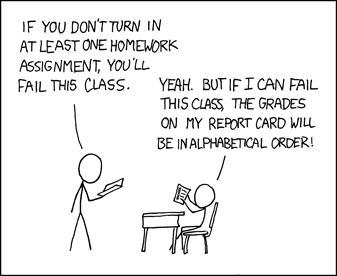
\includegraphics[totalheight=6cm]{bilder/XKCD/priorities}
\end{center}

		\end{multicols}

		\vfill
		\begin{center}
			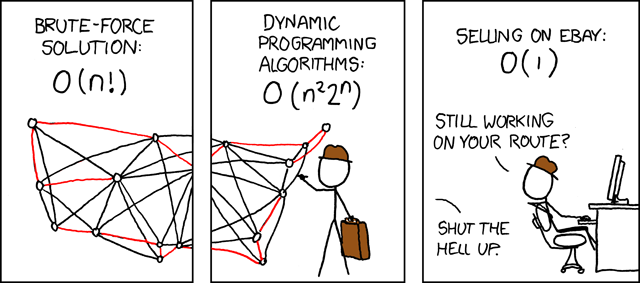
\includegraphics[width=\textwidth]{bilder/XKCD/travelling_salesman}
		\end{center}
		\vfill
	\newpage

	\section{Spezielles im Bachelor}
		\label{bachelor}
		\begin{multicols}{2}
		\subsection{Eure Veranstaltungen im ersten Bachelor-Semester}
	Um euch einen kleinen Vorgeschmack auf die Themen zu geben, die euch im ersten Semester beschäftigen werden, gibt es hier einen Überblick:

	\nottoggle{winter}{Je nach euren Vorkenntnissen kann es auch sinnvoll sein, Programmieren 2 oder Technische Informatik 2 zu belegen. Bevor ihr euch dazu entscheidet, solltet ihr euch aber auf jeden Fall durch uns beraten lassen.}{}

\tocheck{0}{Vorlesungsbeschreibungen mit Empfehlungen abgeleichen}

\iftoggle{winter}{
	% !TEX root = ../../../1-te.tex

\subsubsection{Algorithmen und Datenstrukturen}
	\textit{Prof. S\'andor Fekete}
	Diese Vorlesung vermittelt Programmiersprachenunabhängige Algorithmen und Konzepte wie Bäume, Listen oder Stacks. Wer nicht weiß, was sich hinter diesen Begriffen verbirgt, sollte auf keinen Fall die Übungen verpassen.
	% !TEX root = ../../../1-te.tex

\subsubsection{Programmieren 1}
	\textit{Dr. Werner Struckmann}
	In Programmieren 1 geht es um die Programmierung mit Java. Diese Vorlesung eignet sich vorallem für das Home Studium, da sie viele Übungsaufgaben bietet. In Programmieren 2 werden weitere tiefer gehende Programmiertechniken vermittelt. Wer sich schon gut in Java auskennt, kann Programmieren 1 und Programmieren 2 auch im selben Semester machen.
	% !TEX root = ../../../1-te.tex

\subsubsection{Lineare Algebra}
	\textit{Dr. Wolfgang Marten}
	Hier geht es um Vektoren und Matrizen, sowie ein wenig Gruppentheorie. Die Übungen sind zwar nicht immer einfach, geben aber einen sehr guten Ausblick auf die Klausur.
	\subsubsection{Diskrete Mathematik}
	\textit{Prof. Arnfried Kemnitz und PD JP Bode}
	Diskrete Mathematik handelt von allem, was mit ganzen Zahlen zu tun hat: Fibbonacci-Zahlen, Primzahlen, Modulorechnung, usw. Es werden die wichtigsten Mathemaischen Grundlagen vermittelt, unter anderem in Logik, Kombinatorik, Zahlentheorie und Algebra. Die kleinen Übungen sind hier eine sehr gute Vorbereitung auf die Hausaufgaben und die Klausur.
	\subsubsection{Theoretische Informatik 1}
	\textit{Dr. Jürgen Koslowski}
	Hier geht es um formale Sprachen und Automatentheorie. Klingt theoretisch und mathelastig? Ist es auch. Nicht gleich aufgeben, wenn man in der Vorlesung nicht mitkommt, die kleinen Übungen helfen beim Verständnis und bei der Klausurvorbereitung. Sie ist regulär für das dritte Semester vorgesehen, wer es sich zutraut kann sie aber schon im ersten hören und sich damit den Stundenplan im dritten Semester ein wenig freihalten. 
	\subsubsection{Mathewahlpflicht}
%	\textit{N.N.} 
Ihr müsst insgesamt zwei Module zu je fünf Credits
	im Mathe-Wahlpflichtbereich einbringen. Dabei wird eine Vorlesung im Wintersemester und zwei
	Vorlesungen im Sommersemester	angeboten:
	\begin{itemize}
	  \item Sommersemester: 
	    \begin{itemize} 
	      \item Algebra für Informatiker: Hier gehts um grundlegende
		algebraische Strukturen (Mengen, Gruppen, Monide etc). Diese sind insbesondere für die
		theoretische Informatik von großer Bedeutung.
	      \item Einführung in die Stochastik für Informatiker: Die
		Vorlesung behandelt die Grundlagen der
		Wahrscheinlichkeitstheorie (Laplace- Experimente,
		Erwartungswerte, Zufallsvariablen etc.). 
	    \end{itemize}
	  \item Wintersemester: 
	    \begin{itemize}
	      \item Einführung in die Numerik für Informatiker: Hier
		werden Verfahren zum Lösen numerischer Probleme
		behandelt. 
%	      \item Statistische Verfahren für Informatiker: Hier geht
%		es um statistische Probleme und wie man sie lösen kann.
%		Achtung: Die Vorlesung baut auf  ,,Einführung in
%		die Stochastik'' auf und setzt deren Inhalte voraus! Sie wird jedoch derzeit nicht angeboten.
	    \end{itemize}
	\end{itemize}
	Bei der Auswahl geht ihr am Besten so vor, dass ihr euch erstmal
	in alle gerade angebotenen reinsetzt und dann die behaltet, mit der ihr besser
	klarkommt. Generell gilt aber bei mathematischen Vorlesungen: Es
	gibt im Allgemeinen kein aktuelles Skript, wer nichts verpassen
	will, muss in der Vorlesung mitschreiben. Auch können die
	Hausaufgaben gerne mal umfangreicher werden, bereiten aber dafür
	sehr gut auf die Klausur vor. Dranbleiben und sich nicht
	entmutigen lassen ist alles :)
}{
	% !TEX root = ../../../1-te.tex

\subsubsection{Einführung in die Logik}
	\textit{Prof. Koslowski}
	Die Vorlesung behandelt die Grundlagen der formalen Logik, mit einen starken Fokus auf Aussagen- und Prädikatenlogik. Die Hausaufgaben sind dabei teilweise sehr zeitaufwändig, aber dafür eine gute Klausurvorbereitung. Dabei ist das Skript sehr hilfreich.
	% !TEX root = ../../../1-te.tex

\subsubsection{Analysis}
	\textit{Dr. Wolfgang Marten}
	Hier geht es um Differential- und Integralrechnung, sowie Grenzwerte. Die Übungen sind zwar nicht immer einfach, geben aber einen sehr guten Ausblick auf die Klausur. Die Übungsaufgaben sollte man umbedingt machen, wenn man vorhat die Klausur zu bestehen.
	\subsubsection{Computernetze 1}
	\textit{Prof. Lars Wolf}
	Hier lernt man die grundlegende Funktionsweise von Netzwerken kennen. Für die Klausur sollte man auf gar keinen Fall die Übungen verpassen. Interessiert man sich über die Vorlesung hinaus für das Thema, sollte man in die Bücher von Andrew S. Tanenbaum schauen.
	\subsubsection{Mathewahlpflicht}
%	\textit{N.N.} 
Ihr müsst insgesamt zwei Module zu je fünf Credits
	im Mathe-Wahlpflichtbereich einbringen. Dabei wird eine Vorlesung im Wintersemester und zwei
	Vorlesungen im Sommersemester	angeboten:
	\begin{itemize}
	  \item Sommersemester: 
	    \begin{itemize} 
	      \item Algebra für Informatiker: Hier gehts um grundlegende
		algebraische Strukturen (Mengen, Gruppen, Monide etc). Diese sind insbesondere für die
		theoretische Informatik von großer Bedeutung.
	      \item Einführung in die Stochastik für Informatiker: Die
		Vorlesung behandelt die Grundlagen der
		Wahrscheinlichkeitstheorie (Laplace- Experimente,
		Erwartungswerte, Zufallsvariablen etc.). 
	    \end{itemize}
	  \item Wintersemester: 
	    \begin{itemize}
	      \item Einführung in die Numerik für Informatiker: Hier
		werden Verfahren zum Lösen numerischer Probleme
		behandelt. 
%	      \item Statistische Verfahren für Informatiker: Hier geht
%		es um statistische Probleme und wie man sie lösen kann.
%		Achtung: Die Vorlesung baut auf  ,,Einführung in
%		die Stochastik'' auf und setzt deren Inhalte voraus! Sie wird jedoch derzeit nicht angeboten.
	    \end{itemize}
	\end{itemize}
	Bei der Auswahl geht ihr am Besten so vor, dass ihr euch erstmal
	in alle gerade angebotenen reinsetzt und dann die behaltet, mit der ihr besser
	klarkommt. Generell gilt aber bei mathematischen Vorlesungen: Es
	gibt im Allgemeinen kein aktuelles Skript, wer nichts verpassen
	will, muss in der Vorlesung mitschreiben. Auch können die
	Hausaufgaben gerne mal umfangreicher werden, bereiten aber dafür
	sehr gut auf die Klausur vor. Dranbleiben und sich nicht
	entmutigen lassen ist alles :)
	% !TEX root = ../../../1-te.tex

\subsubsection{Programmieren 2}
	\textit{Dr. Werner Struckmann}
	In Programmieren 1 (jährlich im Wintersemester) geht es um
	grundlegende Konzepte der Programmierung am Beispiel von Java.
	Darauf aufbauend wird in Programmieren 2 (jährlich im
	Sommersemester) die Implementierung von Algorithmen und
	Datenstrukturen geübt. Hat man schon gute Vorkenntnisse in einer
	Programmiersprache (etwa durch eine Ausbildung zum
	Fachinformatiker o.Ä.) kann man sich durchaus auch schon im 1.
	Semester an Programmieren 2 versuchen, die Reihenfolge ist NICHT
	vorgeschrieben. 
	% !TEX root = ../../../1-te.tex

\subsubsection{Technische Informatik 2}
	\textit{Prof. Rolf Ernst}
	Das Modul besteht aus Technischer Informatik 1 und 2 und endet
	mit einer Kombiklausur aus beiden Veranstatungen, die
	Reihenfolge in der man diese besucht ist egal, da die
	Inhalte relativ unabhängig voneinander sind.
	Die Vorlesung zu Technischen Informatik 2 orientiert sich
	weitgehend an dem Lehrbuch \enquote{Logic and Computer Design
	Fundamentals – 4th edition} von M. Mano und Ch. Kime, welches
	gleichzeitig als Skript gilt. Das Buch findet man in
	ausreichender Anzahl in der UB. Die kleinen Übungen sind als
	Klausurvorbereitung zu empfehlen, ersetzen aber nicht das eigene
	Nacharbeiten. Wichtig: Belegt man Technische Informatik 2 schon
	im 1. Semester, ist dies nur sinnvoll, wenn man auch Technische
	Informatik 1 im 2. Semester hört, um die Kombiklausur
	mitzuschreiben. Man sollte sich also gut überlegen, wie weit man
	sich da schon festlegen möchte! Andererseits hat man dann im
	zweiten Semester schon ein relativ dickes Modul abgeschlossen,
	was ja auch nicht verkehrt ist.
}

		% !TEX root = ../../1-te.tex

\subsection{Studienplan}
	\label{bach_studienplan}
	\tocheck{5}{Stimmt die Anzahl Pflichtveranstaltungen noch? Mit aktuellem Stundenplan abgleichen!}
	Wie du wahrscheinlich bereits in deinem Stundenplan festgestellt hast, musst du im ersten Semester \iftoggle{winter}{vier}{vier} Pflichtveranstaltungen hören. Doch die Bezeichnung Pflichtverantstaltung sagt bloß aus, dass du die Veranstaltung \emph{irgendwann} einmal hören musst, um deinen Bachelor abzuschließen. Die zeitliche Abfolge der Veranstaltungen darfst du aber selbst festlegen. Der Fakultäts-Musterstudienplan bietet hier eine gute Orientierungsmöglichkeit. Du musst dich aber nicht daran halten. Niemand zwingt dich eine Veranstaltung zu hören oder hält dich davon ab. Du kannst dich eigentlich in jede Vorlesung setzen, auch ohne hinterher an der Prüfung teilnehmen zu müssen -- allerdings gibt es dann auch keine Punkte dafür. Hier bieten sich zum Beispiel Module aus dem Wahlplichtbereich Informatik an, die eventuell nur alle 2 Jahre angeboten werden und über mehrere Semester gehen. Bei den (Pflicht-)Modulen der Informatik musst du jedoch beachten, dass einige Module auf anderen aufbauen. Zum Beispiel sollten Programmiergrundlagen in den ersten zwei Semestern erarbeitet werden und mit Theoretische Informatik II wirst du dich schwer tun, wenn du TheoInf I nicht gehört hast.

	Damit sich dein Studium nicht unnötig verlängert, solltest du darauf achten, in jedem Semester rund 30 Leistungspunkte zu erwerben.

		% !TEX root = ../../1-te.tex

\xkcd{width=.9\columnwidth}{fixing_problems}

\subsection{Studienplanung im Bachelor}

Wie geht das eigentlich, studieren?

Wie du lernst, studierst, lebst; ob du brav mitschreibst oder öfter mal ausschläfst kannst und musst du selbst entscheiden. Wann du die vorgeschriebenen Lehrveranstaltungen belegst, liegt ebenfalls in deinem eigenen Ermessen, allerdings: Nachdem bis auf sechs Ausnahmen klar festgelegt ist was du studieren musst, ergibt sich eine sinnvolle Reihenfolge, da beispielsweise fortgeschrittenes Programmieren ohne Kenntnis von Algorithmen schlicht nicht möglich ist. Nichtsdestotrotz hast du Spielraum, das Studium an deine persönliche Situation anzupassen.


Du wohnst noch zu Hause und brauchst nicht arbeiten? Prima, mach noch \iftoggle{winter}{Theoretische Informatik 1}{Technische Informatik oder Computernetze} im 1. Semester. Du hast ein Kind und musst nebenbei auch noch arbeiten? Kein Problem, sprich dich mit deinem Mentor ab und mach ein Teilzeitstudium. Die konkreten Vorschriften zum Studium findest du in der Prüfungsordnung.

\tocheck{5}{Stimme die Credit-Anzahlen noch mit der BPO überein (sprich, gab es eine neue BPO)?}

In kurz: Grundsätzlich musst du Veranstaltungen im Wert von 180 Credit Points (CP) erfolgreich absolvieren, davon 130 CP im Bereich Informatik, 35 CP in Mathematik, 10 CP für dein Nebenfach\footnote{Bei Belegung des Nebenfachs \enquote{Betriebswirtschaftslehre} abweichend davon 12 CP} und 5 CP für Schlüsselqualifikationen. 

\tocheck{5}{Beschreibung der Musterstudienpläne aktuell?}

Um dir einen sinnvollen Weg durchs Studium zu ermöglichen, gibt es von der Fakultät den Musterstudienplan, der versucht, Überschneidungen der Veranstaltungen zu vermeiden. %Es gibt aber auch noch Alternativstudienplan der Fachgruppe, die in bestimmten Situationen sinnvoll sein können. 

\tocheck{5}{Neue und korrekte Musterstudienpläne, die das IT-Sec-Problem beachten!}

Normalerweise würden wir dir an dieser Stelle alternative Musterstudienpläne vorstellen, um zu zeigen, dass auch andere Herangehensweisen an das Studium möglich sind. Leider gibt es aufgrund der neuen Bachelor-Prüfungsordnung noch eine \enquote{Bug} in der Belegungslogik: Um \emph{Einführung in die IT-Sicherheit} zu schreiben, musst du erst \emph{Computernetze 1} und \emph{Betriebssysteme} bestanden haben. Mit dieser Belegungslogik lässt sich kein sinnvoll in 6 Semestern studierbarer Plan erstellen.

Daher empfehlen wir euch, die Ohren offen zu halten und abzuwarten, bis eine Lösung gefunden wird. Die Fachgruppe hält euch auf dem Laufenden. Aktuelle Informationen bekommt ihr auf dem Treffen zum Stundenplanbau, oder bei einem Besuch im Fachgruppenraum der FG Informatik.

%Auf den folgenden Seiten findest du die erwähnten Pläne. Der erste ist der Musterstudienplan der Fakultät. Der zweite Musterstudienplan wurde durch die Fachgruppe erstellt, um einige Probleme mit dem durch die Fakultät bereitgestellten Musterstudienplan zu adressieren. So liegt im Plan der Fakultät die Pflichtvorlesung \emph{Einführung in die IT-Sicherheit} im fünften Semster. Das führt dazu, dass sich das Studium bei Nichtbestehen des Moduls zwingend um ein Semester verlängert, da man die Bachelorarbeit erst nach Bestehen aller Pflichtmodule anmelden kann

%Der zweite Musterstudienplan zieht einige Veranstaltungen nach vorne, sodass weniger Vorlesungen parallel zur Bachelorarbeit im sechten Semster liegen. Diesen Plan empfehlen wir dir allerdings nur, wenn du dir einen gewissen Mehraufwand gerade auch in den ersten Semstern zutraust. Weitere Informationen bekommst du auf dem Treffen zum Stundenplanbau nach dem Erstsemesterfrühstück oder bei einem Besuch im Fachgruppenraum der FG Informatik.

% So liegt im Plan der Fakultät z.\ B. ein Semester zwischen den Vorlesungen Programmieren I und Programmieren II. Wir halten es nicht für sinnvoll, aufeinander aufbauende Vorlesungen voneinander zu trennen und legen daher Programmieren II direkt ins 2. Semester. 

%Außerdem soll das Teamprojekt nach dem Musterstudienplan der Fakultät parallel zur Bachelorarbeit im 6. Semester gemacht werden. Da Projekte erfahrungsgemäß mit einem relativ hohen Arbeitsaufwand verbunden sind, empfehlen wir, das Projekt schon früher durchzuführen, damit man sich im 6. Semester voll auf die Bachelorarbeit konzentrieren kann. Weitere Informationen, oder Erfahrungen bekommt ihr auf dem Treffen zum Stundenplanbau, oder bei einem Besuch im Fachgruppenraum der FG Informatik.

% Der zweite Musterstudienplan gibt eine Orientierung, falls man das Fach Technische Informatik vorverlegen möchte. Der dritte Plan zeigt die Möglichkeit das Fach Theoretische Informatik vorzuverlegen. Bei beiden Plänen wurden zusätzliche Vorlesungen umgelegt, damit der Lernaufwand möglichst ausgeglichen bleibt. Theoretische Informatik und Technische Informatik bauen auf die Kenntnisse aus den Vorlesungen der ersten beiden Semester auf. Die Umlegung dieser Kurse nach vorne ist somit für diejenigen eine Möglichkeit, die schon vorher Kenntnisse gesammelt haben. Weitere Informationen, oder Erfahrungen bekommt ihr auf dem Treffen zum Stundenplanbau nach dem Erstsemesterfrühstück, oder bei einem Besuch im Fachgruppenraum der FG Informatik.

\nottoggle{winter}{Ein grundsätzliches Problem des Studienbeginns im Sommersemester ist, dass viele Fächer auf den Inhalten der Mathevorlesungen des Wintersemesters aufbauen. Je nach euren Vorkenntnissen kann es daher sinnvoll sein, stattdessen andere Fächer zu belegen. Da eine pauschale Aussage aber nicht möglich ist, sondern viel vom Einzelfall abhängt, führen wir mit euch eine Veranstaltung zur Studienplanung durch. Diese solltest du nicht verpassen!}{}

Du bist nicht mehr in der Schule, du hast nun Freiheiten. Nutze sie weise und studiere so, wie du es für richtig hältst!

		\end{multicols}
		% !TEX root = ../../1-te.tex

\tocheck{1}{Aktuelle Musterstudienpläne der FG einfügen}
\label{musterstudienplan}

\iftoggle{winter}{
	\begin{minipage}[H]{1.0\linewidth}
	\begin{center}
	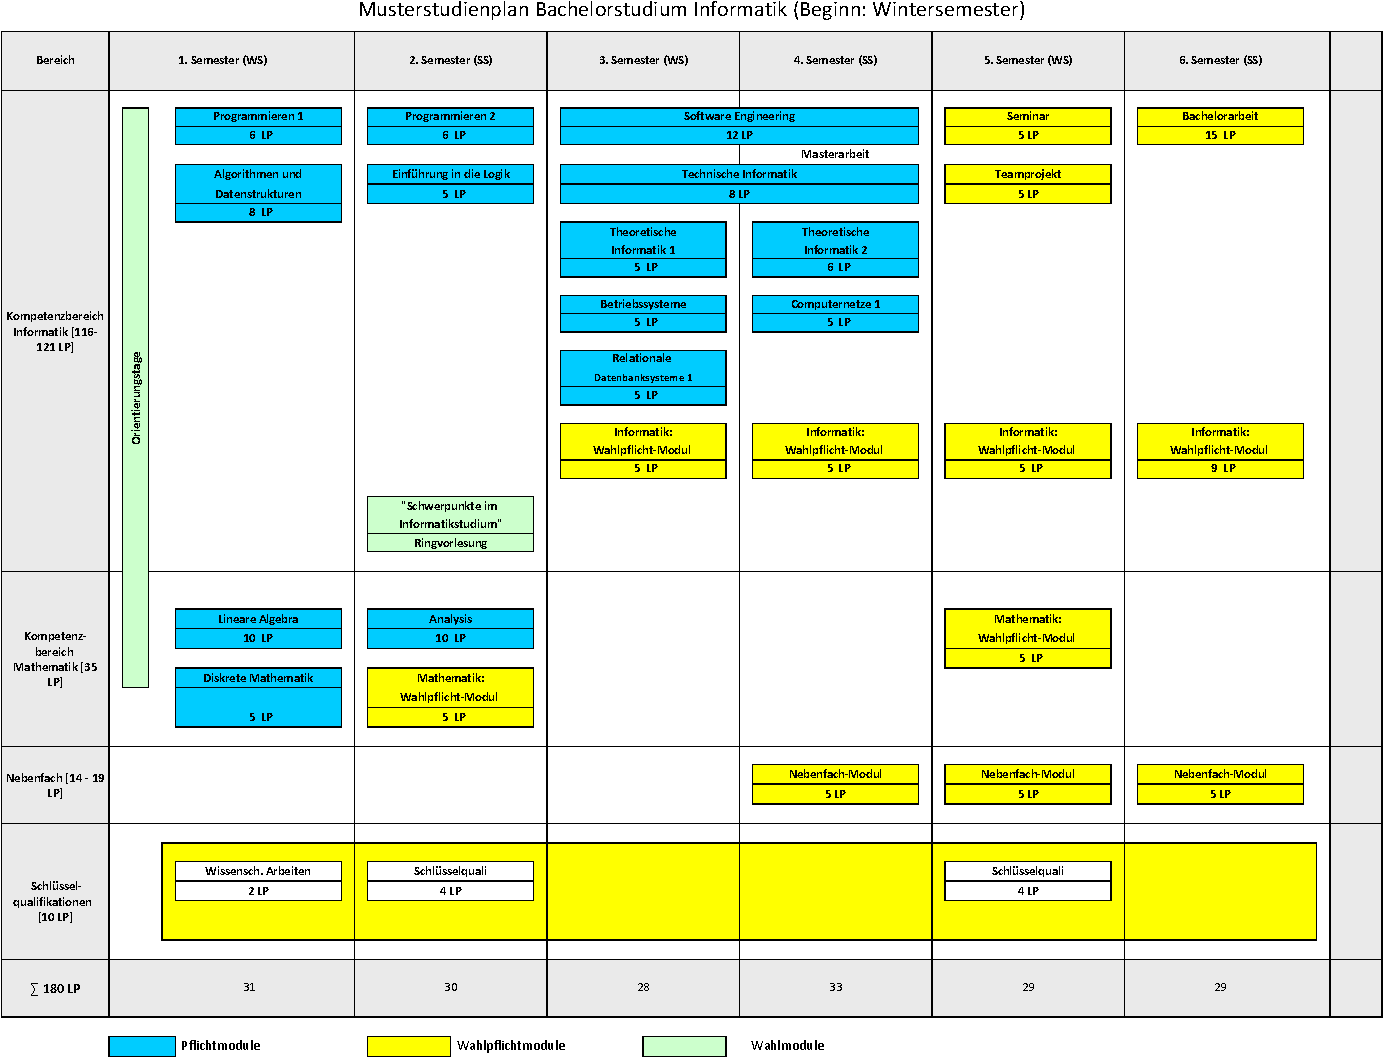
\includegraphics[angle=90, totalheight=\textheight, width=\textwidth ]{bilder/studienplan_bsc_ws/muster_erste_ws-crop}
	\end{center}  
	\end{minipage}
	\newpage

	\begin{minipage}[H]{1.0\linewidth}
	\begin{center} 
			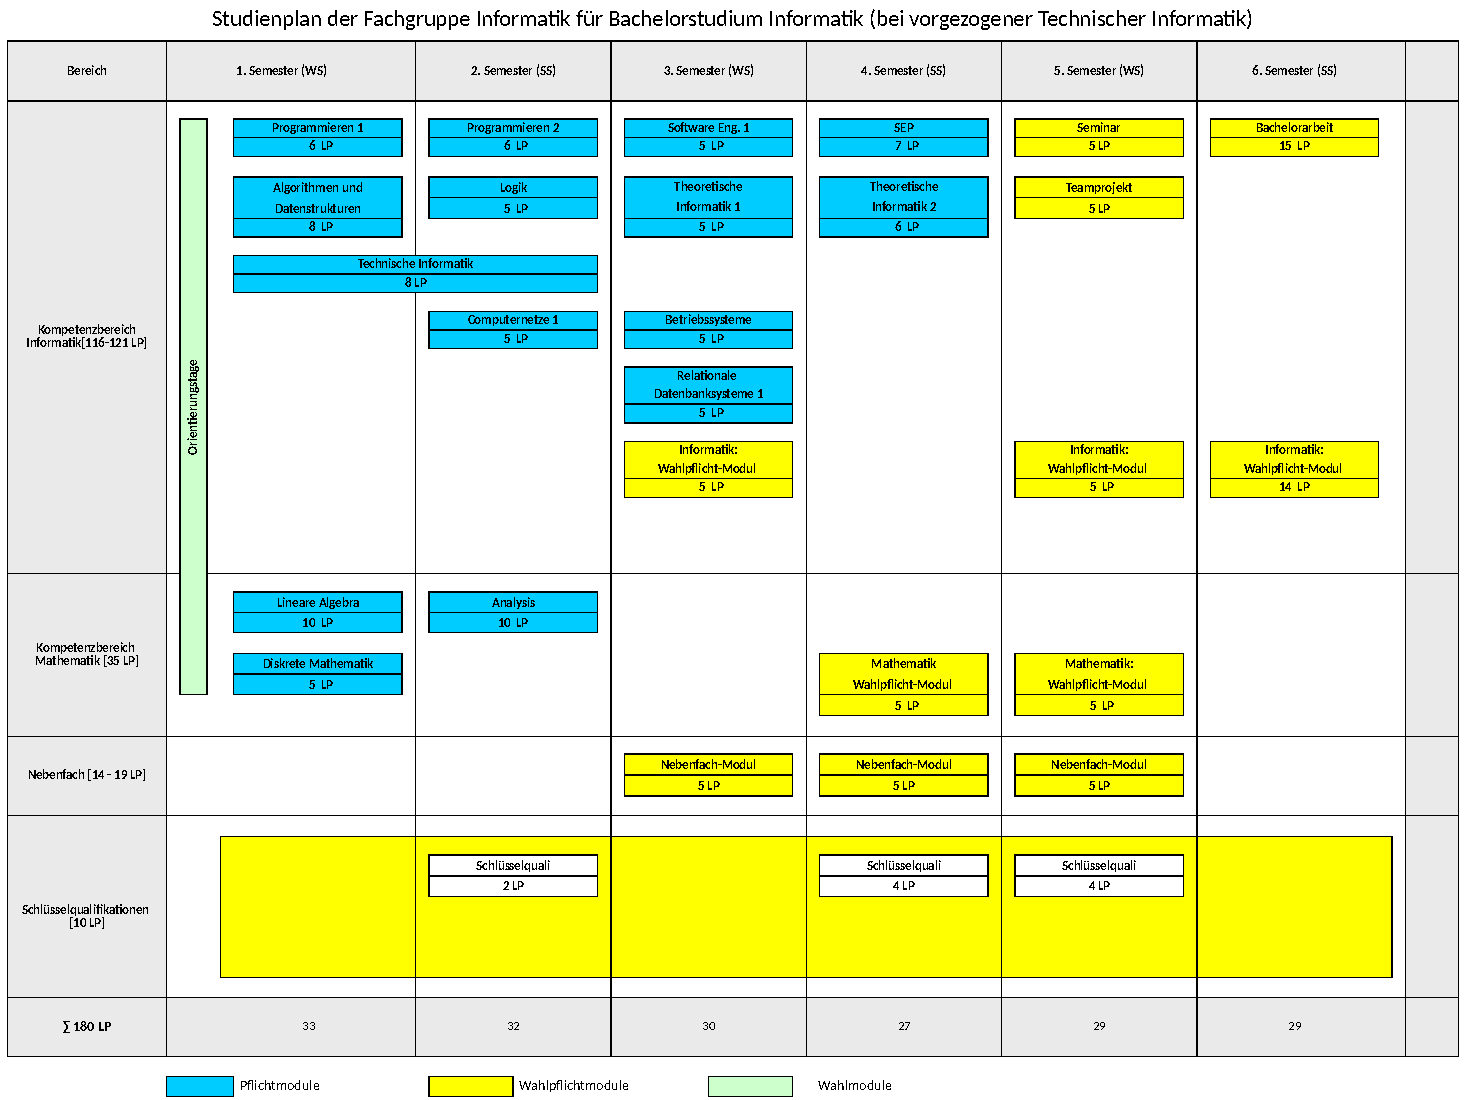
\includegraphics[angle=90, height=\textheight, width=\textwidth ]{bilder/studienplan_bsc_ws/ws2015/BScInformatikWS1516-fginfo-tech_scissored}
			\label{studienplan_tech}
	\end{center}
	\end{minipage}
	\newpage

	\begin{minipage}[H]{1.0\linewidth}
	\begin{center} 
			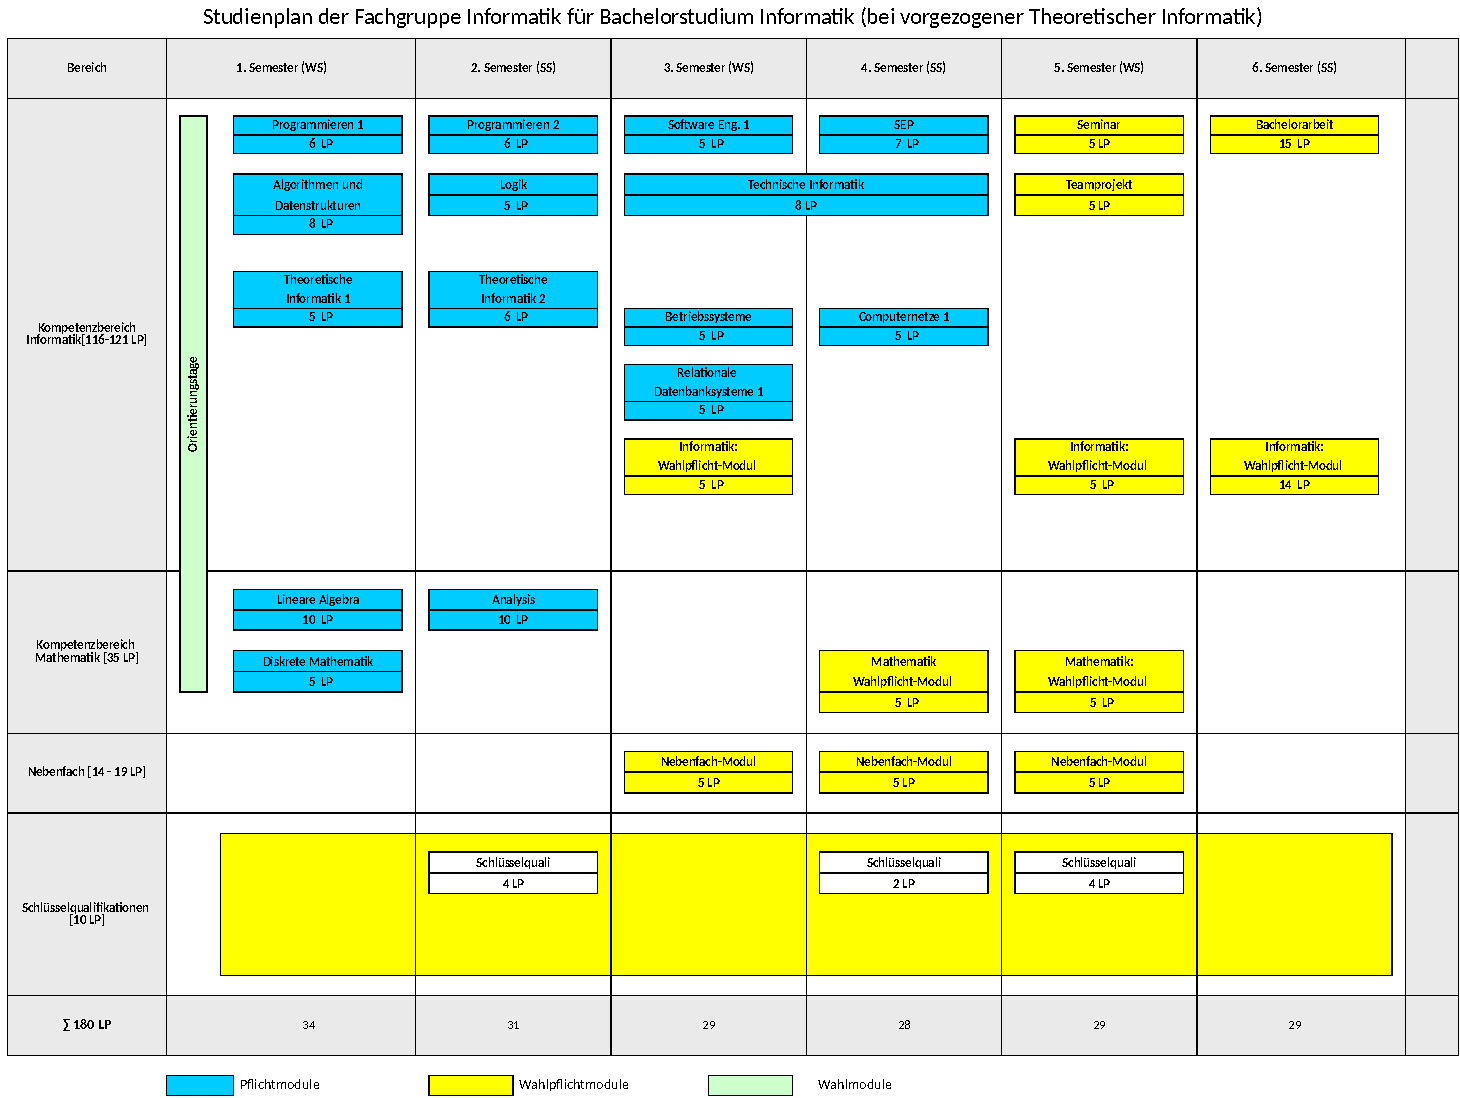
\includegraphics[angle=90, totalheight=\textheight, width=\textwidth ]{bilder/studienplan_bsc_ws/ws2015/BScInformatikWS1516-fginfo-theo_scissored}
			\label{studienplan_theo}
	\end{center}
	\end{minipage}
}{
	\begin{minipage}[H]{1.0\linewidth}
		\begin{center}
		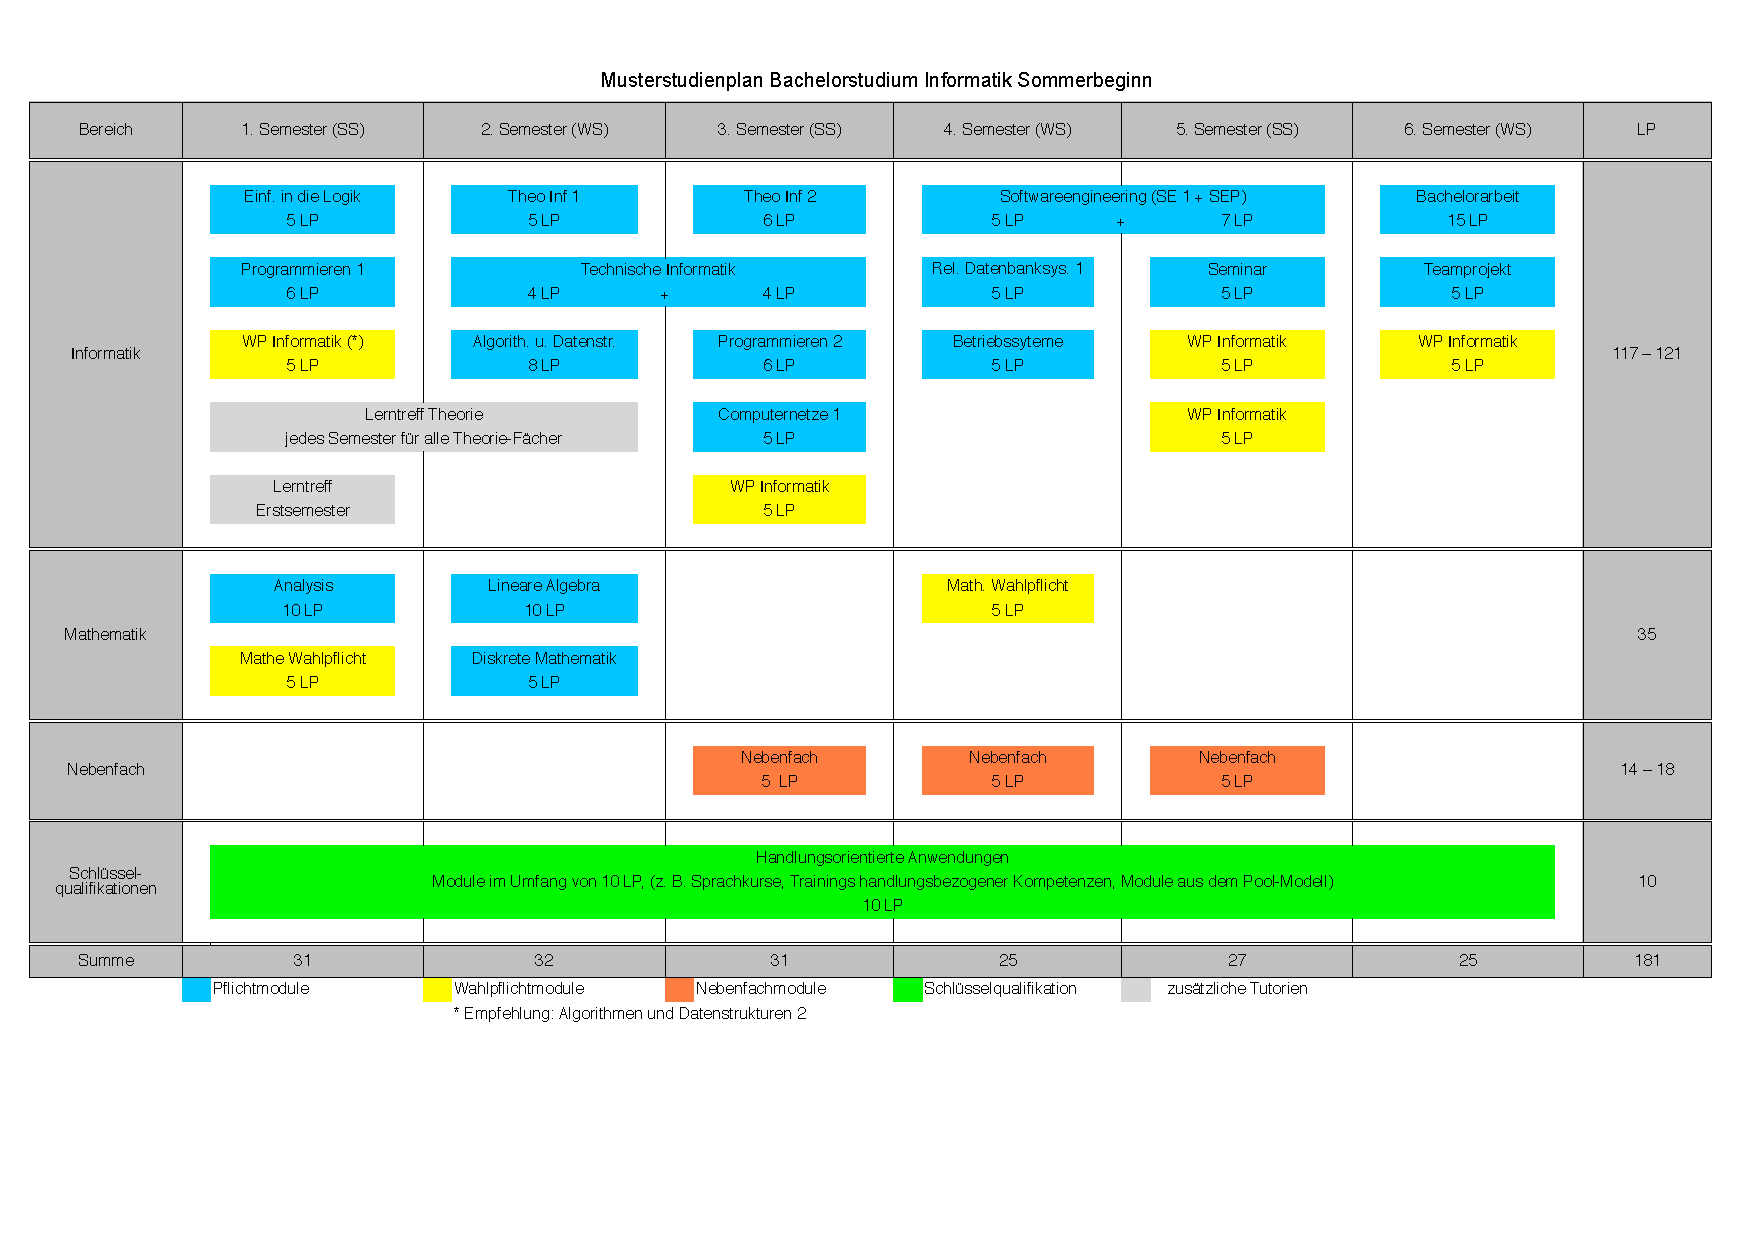
\includegraphics[angle=90, totalheight=\textheight]{bilder/studienplan_bsc_ss/Musterstudienplan_SoSe16.pdf}
		\end{center}  
	\end{minipage}

	\begin{minipage}[H]{1.0\linewidth}
		\begin{center}     
		\label{musterstudienplan}
		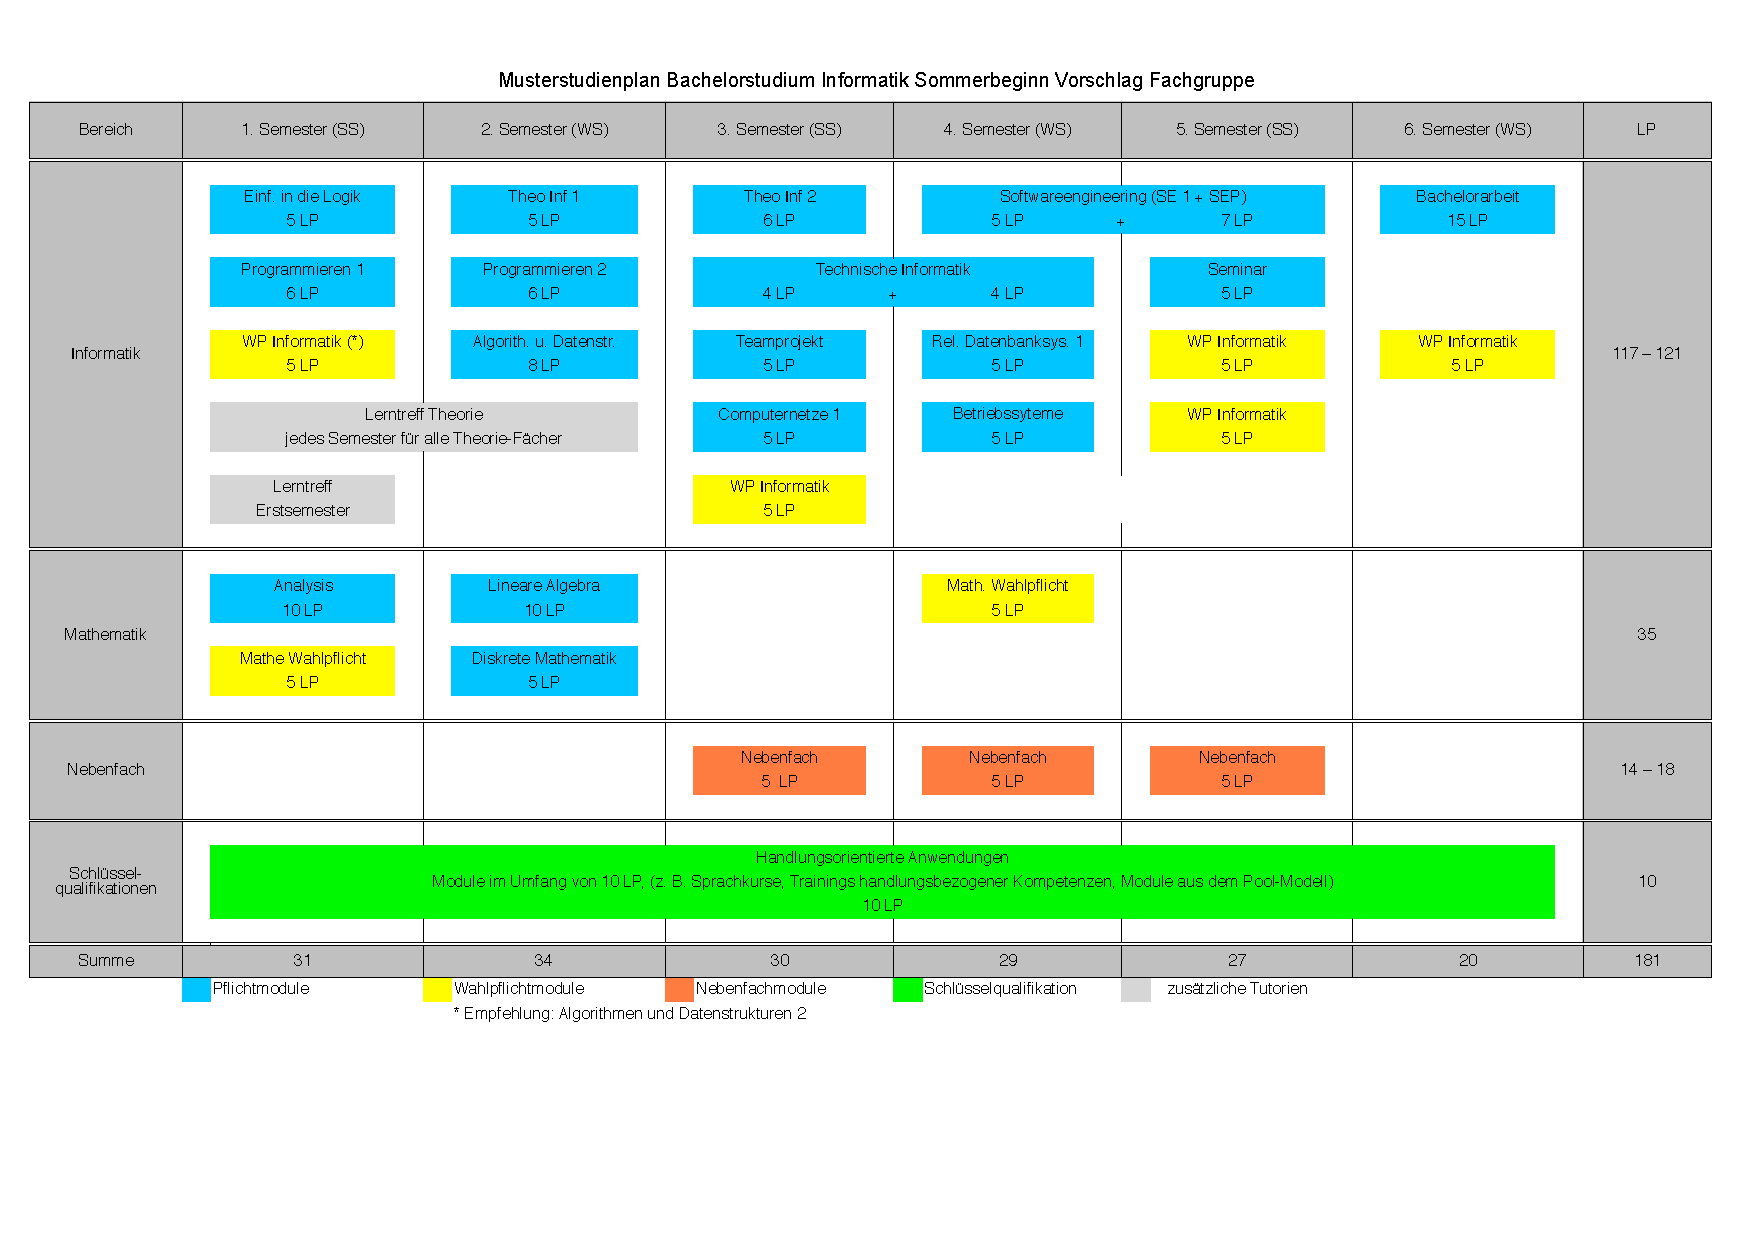
\includegraphics[angle=90, totalheight=\textheight]{bilder/studienplan_bsc_ss/Musterstudienplan_SoSe16_Empfehlung_FG.pdf}
		\end{center}  
	\end{minipage}
}

	%\newpage

	\section{Spezielles im Master}
		\label{master}
		% !TEX root = ../../1-te.tex

\begin{minipage}{1.0\linewidth}
	\begin{center}     
 		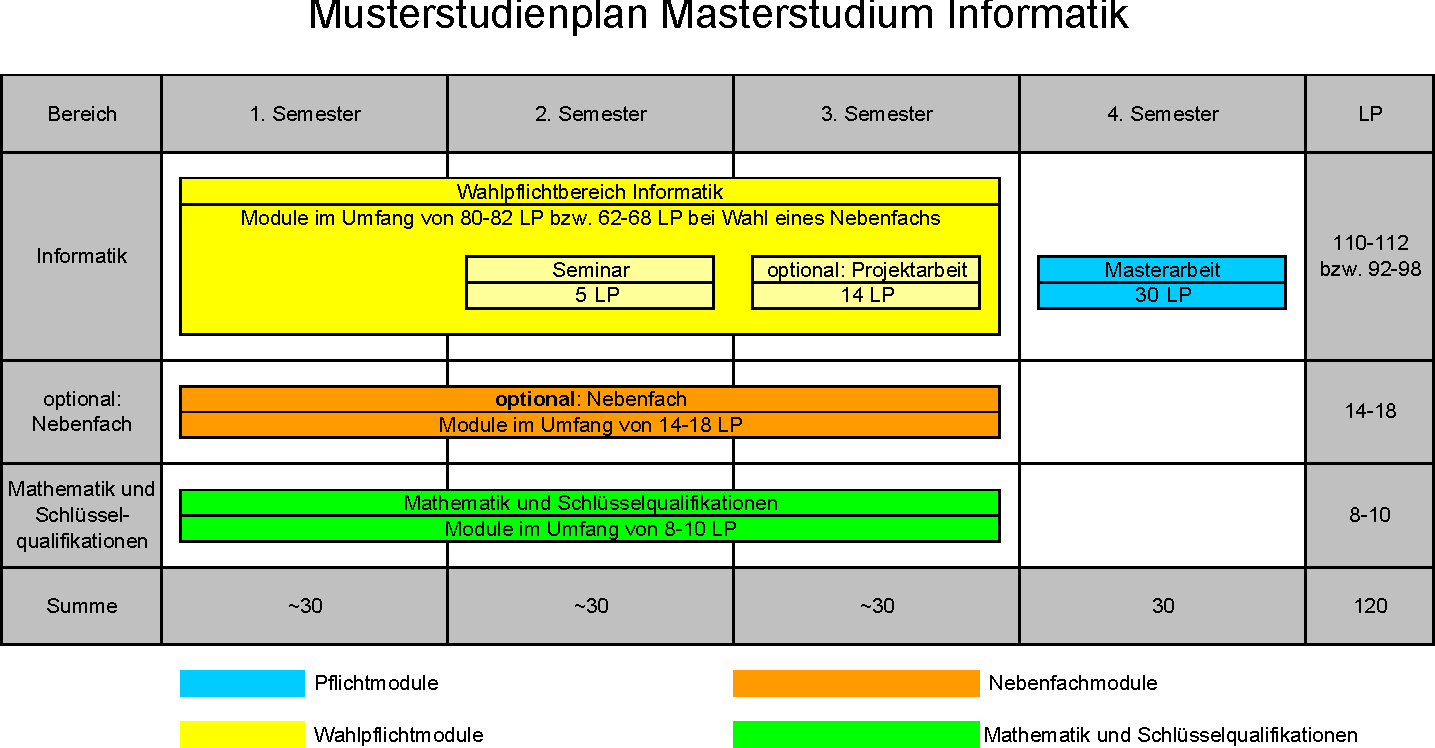
\includegraphics[width=\textwidth]{bilder/studienplan_msc/Musterstudienplan_MSc.pdf}
	\end{center} 
\end{minipage}

\begin{multicols}{2}
	Wer seinen Bachelor nicht in Braunschweig erworben hat, steht im ersten Mastersemester vielen kleinen und mittelgroßen Schwierigkeiten gegenüber.

	\subsection{Unterschiede zwischen den Bachelor-Abschlüssen}
		Eventuell hat dein bisheriger Abschluss dir mehr als 180 Credit Points eingebracht -- genau so viele hättest du nämlich in einem Bachelor an dieser TU erreicht. Es ist theoretisch möglich, solche überschüssigen CPs auf den Master anzurechenen, wenn man von seiner alten Hochschule bestätigt bekommt, dass sie für den Bachelor nicht verwendet wurden. Dann kann man die Anerkennung dieser CPs beim Prüfungsausschuss beantragen, wobei man möglichst schlüssig begründen muss, warum diese Vorlesungen dem TU-BS-Master würdig sein sollen.

		Selbst bei gleicher Anzahl an CP ist der Bachelor an jeder Hochschule ein wenig anders. Zwischen Universitäten in Deutschland herrscht eine formale Übereinkunft über die Inhalte des Bachelor-Studiums Informatik. 

		Falls du von einer Nicht-Universität (z.B. Fachhochschule) oder aus einem Studiengang der nicht exakt \emph{Informatik} heißt kommst oder dein Abschluss kein Bachelor of Science ist, dann kann es durchaus sein, dass du bei gewissen Unterschieden Zulassungsauflagen bekommst, um diese zu beheben.

	\subsection{Zulassungsauflagen}
	\label{auflagen}
	Ob du Zulassungsuflagen bekommst, steht in einem der ersten Briefe, die du von der TU erhältst, heb diesen Brief gut auf! Wenn du keine solchen Zulassungsauflagen hast, kannst du diesen Abschnitt überspringen.

	Es handelt sich dabei um Fächer aus dem Informatik-Bachelor, die du zusätzlich zu den Master-Fächern belegen musst -- sie gehen aber nicht in die Masternote oder CP ein und müssen innerhalb des ersten Jahres bestanden und im I-Amt nachgewiesen werden, sonst droht die Exmatrikulation.

	Der Sinn hinter den Auflagen ist es, Differenzen zum TU-BS-Bachelor auszugleichen, d.h. Inhalte nachzuholen, die in deiner bisherigen Ausbildung zu kurz kamen oder ganz fehlten, und hier wichtige Grundlage des Masterstudiums sind.

	Es ist möglich, zu Semesterbeginn freiwillig an einer mündlichen Prüfung teilzunehmen. Wird diese bestanden, dann ist die Auflage erfüllt, falls nicht, muss wie gehabt die Klausur belegt werden. Auch wird in den meisten Fächern die Hausaufgabe nicht mehr verpflichtend sein, um an der Klausur teilzunehmen.

	Viele Fragen zu den Zulassungsauflagen sind unter \fginfoUrl $\rightarrow$ FAQ dokumentiert und nach bestem Wissen und Gewissen beantwortet. Falls du eine Auflage erhalten hast, die dir fragwürdig erscheint oder du sonst irgendwelche Fragen dazu hast, wende dich am besten an den Fachgruppenrat.

	Ratsam ist es auch, mit den anderen Ersties in deinem Jahrgang zu sprechen und zu vergleichen, wie deren Auflagen aussehen bzw. welche Schritte diese gerade erwägen. 

	\subsection{Selbstständiges Nachlernen von Bachelor-Fächern}
		Vielleicht hat dein Bachelor eine andere Ausrichtung gehabt als die TU und somit in manchen Bereichen klare Wissenslücken hinterlassen. Wenn du das Gefühl hast, dass dir Wissen fehlt, das im Braunschweiger Bachelor vermittelt wurde, kannst du dich natürlich auch freiwillig in jede Bachelor-Vorlesung oder Übung hineinsetzen -- Punkte gibts dafür normalerweise keine. Aber egal was dir aus dem Bachelor fehlt, es finden sich eigentlich genug Master-Fächer, die auch ohne bestimmte Vorkenntnisse, gut schaffbar sind. Einige wenige Master-Vorlesungen beginnen auch mit einer mehrwöchigen Widerholung der Bachelor-Grundlagen. Im Zweifelsfall frage Studierende aus den höheren Semestern oder den oder die Professor/in selbst, welche Vorkenntnisse man wirklich braucht.

	\subsection{Der eigene Stundenplan}
		\label{masterstundenplan}
		Es gibt durchaus Studierende, die mit dem Stundenplanbau kein Problem haben: Sie schauen einige Minuten auf den Gesamstundenplan, es macht Klick, und sie wissen, welche Fächer sie belegen wollen. Andere verbringen bis zu 12 Stunden damit ihren Stundenplan zu bauen.

		Wenn du Zulassungsauflagen hast, haben diese oberste Priorität. Die entsprechenden Vorlesungen und Übungen kannst du ohne großes Nachdenken in deinen Stundenplan eintragen -- außer wenn du die freiwillige mündliche Prüfung bestanden hast.

		Danach kannst du probieren den allgemeinen Stundenplan pro Block durchzugehen und zu entscheiden, welches der dort stattfindenen Fächer für dich interessant klingt. Wenn du so vorgehst, hast du vermutlich am Ende einen Plan mit viel zu vielen Fächern, also deutlich mehr als 30 Credit Points. Und was zu Beginn noch überschneidungsfrei aussieht, kollidiert am Ende vielleicht bei den Übungsterminen. 

		Man muss nicht immer beide Veranstaltungen besuchen: bei manchen Fächern kann man die Übung getrost weglassen, oder den Stoff auch ohne Vorlesung aus Skript und Büchern lernen und nur zur Übung kommen. Manche Institute filmen ihre Vorlesungen auch und machen sie terminunabhängig. Frage am besten höhere Semester nach ihren Erfahrungen mit dem betreffenden Fach.

		\vspace{0.5cm}
		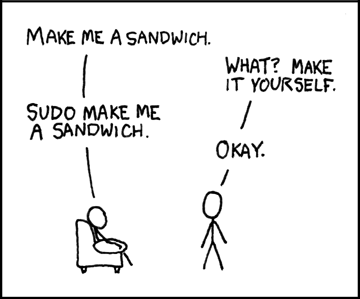
\includegraphics[totalheight=6cm]{bilder/XKCD/sandwich}
	\subsubsection{Hilfe beim Stundenplanbau}
		\tocheck{3}{Wann findet der Workshop diese Jahr statt?}
		Wir bieten seit einigen Semestern zu Beginn Hilfe beim Stundenplanbau an. Dieses Mal findet der Workshop am Mittwoch in der O-Woche um 12:30 Uhr statt. 
\end{multicols}

	\newpage

	\section{Computer und so\ldots}
		\label{computer}
		\section{Computer und so\ldots}
	\label{computer}

\begin{multicols}{2}
	\emph{Informatik hat viel mit Computern zu tun!} - Diesem (Irr-)glauben erliegen zu Anfang des Studiums einige, auch wenn sich inzwischen öfter rumspricht, dass das Studium abstrakter sein kann. Das Informatikstudium ist nicht dafür da,  euch beizubringen, wie man einen Computer bedient. Somit sind diese Seiten eventuell das erste und letzte Mal,  dass euch Infos zu diesem Thema direkt vorgesetzt werden. Natürlich können wir hier nur ein paar Tipps geben und euch darauf hinweisen, wo ihr mehr Infos  findet.

	In Wirklichkeit hängt es seht von deiner Spezialisierung im Studium ab, ob  du den Computer im Studium mehr brauchen wirst als ein Student der Germanistik oder Sozialwissenschaften. Denn die einzigen Inhalte,  die jeder direkt am Rechner lernen und umsetzen muss, sind die Hausaufgaben,  die in Programmieren aufgegeben werden, sowie später noch das SEP und das Teamprojekt. Den Rest der Informatik kannst du evtl. komplett auf dem Papier absolvieren.

	Dennoch sind Computer ein unersetzliches Werkzeug um durchs Studium zu kommen. Und je nach den von dir gewählten Modulen kann sich das oben gesagte auch ins Gegenteil verkehren, so dass du mehr Zeit vorm Rechner als im Bett verbringst.

	Aber heißt dass nun, dass ihr um zu Studieren einen eigenen, top-aktuellen Rechner braucht, und dass ihr absolute PC-Freaks sein solltet? Dem wollen wir auf den nächsten Seiten ein wenig auf den Grund gehen.
\end{multicols}

%\begin{multicols}{2}
	\subsection{Wozu Computer?}
		\subsubsection{Vorlesungen Online}
			Zu den meisten Vorlesungen kann man die Skripte im Internet finden. Für einige Vorlesungen gibt es sogar Ton- oder Videomitschnitte.

			Es gibt auch immer engagierte Studierende, die ihre Vorlesungsmitschriften online stellen. Da diese sehr wahrscheinlich in deinem Semester sind, hilft es, wenn du dich in den Vorlesungen umhörst. Ansonsten ist \url{https://www.clevershit.de} die richtige Anlaufstelle für den Informationsaustausch zwischen Studenten.

		\subsubsection{Organisatorisches ohne Papier}
			Ansonsten gibt es eine Reihe von Informationen, die man nur über das Web bekommt, und mehr und mehr Formalitäten (z.B. die Prüfungsanmeldung) werden auch in die virtuelle Relatität verlagert.

			Desweiteren kannst du dir im Netz einen individuellen Stundenplan zusammenstellen, in Erfahrung bringen, wann die nächsten Klausuren stattfinden, lesen, was es in der Mensa zu essen gibt, endlich herausfinden, wann das Prüfungsamt geöffnet hat,  offene HiWi"~Stellen bei den Instituten finden und vieles mehr.

			Die Webseiten der TU sind ein großer Dschungel, durch den man sich am besten  mit Machete und Googlesuche kämpft. Um an der TU etwas zu finden, solltest du deinem eigentlichen Suchbegriff wahlweise \enquote{tu braunschweig} oder \enquote{site:tu-braunschweig.de} anhängen, und schon hast du gute Chancen zum Ziel zu kommen.

		\subsubsection{Mitschreiben am PC}
			Auf den ersten Blick mag es naheliegen, sich
			während der Vorlesungen Notizen  am Laptop
			anzufertigen. In der Praxis gibt es da aber eine
			Reihe von Problemen, vor denen wir  warnen
			möchten. Es hat schließlich seinen Grund, das
			nur 10\% der Studenten in der Vorlesung am
			Laptop sitzen und davon 90\% diesen nur nutzen,
			um zu zocken: Die meisten Tafelanschriften
			bestehen  aus verschachtelten Formeln,
			fremdartigen Buchstaben und verworrenen
			Zeichnungen. Diese in Echtzeit in den Laptop
			einzuhacken ist eine besondere Kunst, die du mit
			Notepad und Word gar nicht erst probieren
			brauchst. Eine Chance hast du vielleicht mit
			einem Tablet PC, oder wenn du
			\LaTeX\ bereits im Schlaf beherrscht -
			aber wer tut das schon zu Beginn des Studiums?

			In den Vorlesungen, in denen du nicht Tafelweise abschreiben musst, sondern nur hier und da mal etwas notieren, zeigt sich der PC schon als nützlicher. Wenn du ab und zu den Vortrag des Profs damit vergleichen möchtest, was er in sein Skript geschrieben hat, kann dir der mitgebrachte Laptop unter Umständen das Ausdrucken von ein paar hundert Seiten ersparen. Du wirst aber schnell merken, dass es in praktisch keinem der Hörsääle und Seminarräume Steckdosen gibt, und in manchen nichtmals ausreichende WLAN-Signalstärke.

		\subsubsection{Hausaufgaben am PC}
			In vielen Fächern musst du regelmäßig
			Hausaufgaben erledigen und einreichen. Keiner
			erwartet von dir, dass diese mit dem PC gemacht
			werden, es ist also völlig ok sie von Hand zu
			schreiben. Es hat aber auch gewisse Vorteile,
			sie am PC zu schreiben (z.B. mittels \LaTeX) und
			dann auszudrucken. Bei \LaTeX\ handelt es sich
			um ein Satzsystem für wissenschaftliche
			Texte wie Haus- oder Abschlussarbeiten.
			Erwähnenstwert ist die hervorragende
			Unterstützung für den Satz mathematischer
			Formeln und dass dabei mit Befehlen, ähnlich wie
			in HTML gearbeitet wird. Es gibt \LaTeX-Kurse die du im Schlüsselqualifiktationsbereich anrechnen lassen kannst, aber mit den Infos im WWW kann man sich das auch selbst beibringen. Je eher du damit anfängst, desto weniger Probleme hast du später, wenn du damit z.B. deine Abschlussarbeit aufsetzt.

		\subsection{Computer-Pools an der Uni}
			Es ist immer nützlich zu wissen, wo man mal schnell an einen Computer kann. Zumindest ab und zu wirst du die Computer in der Uni benutzen, besonders die Linuxarbeitsplätze in \textbf{PK4.5} oder \textbf{PK4.8}, an denen du die Hausaufgaben für Programmieren abgeben musst.

			\begin{itemize}
				\item[*] Im Erdgeschoss des Altbaus gibt es auf der rechten Seite zwei Computerräume, einen weiter vorne (\textbf{PK4.6}) und einen genau in der Ecke des Gebäudes (\textbf{PK4.5}). Zwei weitere Räume (\textbf{PK4.8} und die \textbf{Datenstation}) findest du im ersten Stock des Altbaus, auch wieder in der rechten Ecke. Die Rechner in \textbf{PK4.5} und \textbf{PK4.8} sind mit Linux ausgestattet. Im ersten Stock gibt es nun auch einen Windowsrechnerraum. Da kann man mal eine Word- oder Powerpoint-Datei ausdrucken, wenn man denn muss.

				\item[*] Reichlich Computer findet man schließlich im Gauß-IT-Zentrum~(GITZ) an der Hans-Sommer-Straße. Das ist der gedrungene, fast würfelförmige, dunkle Klotz hinter dem Elektrotechnik-Hochhaus (\emph{E-Tower}). Hier gibt es mehrere frei zugängliche Räume mit  Linux- und Windowsrechnern. Es gibt hier auch Räume für Medienbearbeitung, wo du etwa Video-Digitalisierer, ein Tonstudio und Rechner mit der Adobe Creative Suite Production Premium nutzen kannst.

				\item[*] Seit 2010 stellt das IBR (Institut für Betriebssysteme und Rechnerverbund) im Raum G40 des Informatikzentrums einen Rechnerraum mit vielen, schnellen Linux-Rechnern  zur Verfügung. Zu diesem CIP-Pool (Computer-Investitions-Programm) bekommt man mit seiner y-Nummer Zutritt. Wenn man Glück hat, funktioniert sogar einer der beiden Drucker in diesem Raum, so dass man zum Drucken nicht das IZ verlassen muss.
			\end{itemize}

		\subsection{Der eigene Rechner}
			Wenn du trotz aller Widrigkeiten planst, dir
			extra für's Studium einen (tragbaren) Rechner
			anzuschaffen, dann hast du hier gleich ein wenig
			Kaufberatung: Viel (Rechen- bzw.
			Grafik-)Leistung brauchst du im Studium  nur für
			sehr wenige spezielle Fachgebiete - das
			einfachste Netbook wird also vermutlich schon
			reichen. Wichtiger ist vielmehr die Akkulaufzeit
			und die WLAN-Empfangsstärke. %a die Här	

		\subsubsection{Welches System?}
			Dir wird auffallen, dass zwar alle Systeme geduldet sind, aber die Linux hier deutlich öfter über den Weg laufen wird als in der freien Wildbahn. Auch wir sind große Linux-Fans und haben deshalb ab Seite \pageref{linux} ein paar Infos dazu zusammengetragen.

			Aber trotz dieser nicht ganz unauffälligen Beeinflussung gilt: Beim Betriebssystem hast du freie Wahl. Sämtliche Software, die du für's Studium brauchen  könntest, gibt es für alle großen Systeme, meist sogar gratis. Für Linux ist eh  praktisch alles frei erhältlich, für Windows spendiert Microsoft den Studenten auch alles außer Office (siehe Seite \pageref{msdnaa}), und auch Apple bringt dich dank satter Studentenrabatte durch Bachelor und Master. 

		\subsubsection{Wege ins Uni-Netz}
			Um den eigenen Rechner ins Netz zu bekommen, stehen die in der Uni WLAN und LAN offen. Zur Konfiguration siehe Seite \pageref{wlan}.

			Für manche Aktivitäten (z.B. den Zugriff auf Prüfungsprotokolle) musst du dich direkt im Uni-Netz befinden. Wenn du und dein Rechner aber gerade zuhause oder sonstwo sind, heißt dass nicht, dass du dich nun physisch auf den Weg machen musst. Mittels VPN kannst du dich virtuell ins Uni-Netz einklinken. Schau einfach mal auf den Seiten des GITZ nach, um mehr zu erfahren.
%\end{multicols}

%\subsection*{\Large{Du bist computers"uchtig, wenn\ldots}}

\begin{enumerate}
\item \ldots du eine Viertelstunde brauchst, um durch deine Bookmarks zu scrollen.
\item \ldots du deinen Lautsprecher aufdrehst, bevor du das Zimmer verl"a"st, damit du das akustische Signal h"orst, wenn eine neue E-Mail eintrifft.
\item \ldots dein Hund eine eigene Homepage hat.
\item \ldots du deine Mutter nicht anrufen kannst, weil sie kein VoIP-Telefon hat.
\item \ldots du deine Mail abrufst, die Meldung kommt: "`No new messages"' - und du sie gleich nochmal abrufst.
\item \ldots du das Geschlecht von dreien deiner besten Freunde nicht kennst, weil sie neutrale Nicknames haben und du sie nie danach gefragt hast.
\item \ldots du morgens um 3 Uhr aufwachst, zum Klo gehst und auf dem R"uckweg am Computer halt machst, um deine Mailbox abzurufen.
\item \ldots du dich t"atowieren l"asst: "`Diesen K"orper betrachtet man am besten mit Mozilla 5.0 oder h"oher"'.
\item \ldots dein Partner sagt, dass das Gespr"ach f"ur eine Beziehung wichtig ist, also kaufst du einen zweiten Rechner und richtest ihm/ihr einen IRC-Client ein.
\item \ldots dir jemand einen Witz erz"ahlt und du mit *lol* antwortest.
\item \ldots du deinen Freunden von einer hei"sen Verabredung erz"ahlst und ihnen verschweigst, dass sie in einem Chatroom stattfindet.
\item \ldots du dir einen Laptop kaufst, um auch auf dem Klo surfen zu k"onnen.
\item \ldots du auf eine Webseite schaust, die voll mit Links von jemand anderem ist, und alle Links bereits in Lila erscheinen.
\item \ldots dich dein Provider bei technischen Schwierigkeiten um deine Hilfe bittet.
\item \ldots du bei \nurl{http://www.wetter.de/} nachschaust, anstatt aus dem Fenster.
\item \ldots Google bei dir anfragt, was noch in ihrer Suchmaschine fehlt.
\item \ldots du deinen Kopf zur Seite beugst, um zu l"acheln.
\item \ldots deine Kaffeemaschine eine eigene IP hat.
\item \ldots du versuchst Texte aus deinem handgeschriebenen Script per copy and paste in ein \LaTeX-Dokument einzuf"ugen.
\item \ldots du keine Kiste mit alten Computerteilen hast, weil z.B. der alte 386er noch als Anrufbeantorter genutzt wird.
\item \ldots du deine HiFi-Anlage "uber einen eigens daf"ur aufgesetzten Webserver steuerst.
\item \ldots du bei vier Webbrowserspielen unangefochten auf Platz 1 stehst.
\item \ldots du wei"st, was man unter\\ \nurl{http://www.google.de/search?&amp;q=5\%5E2\%2B23\%2D3\%21&amp;btnG=Suche&amp;meta=} findet.
\end{enumerate}
 %Veraltet?
\begin{multicols}{2}
\subsection{Gauß-IT-Zentrum}

	Das Rechenzentrum der TU-Braunschweig heißt Gauß-IT-Zentrum oder kurz GITZ. Es bietet euch eine Vielzahl an Diensten an. Manche davon könnt ihr nur vor Ort nutzen, also in der Hans-Sommer-Str. 65, direkt hinter dem ,E-Tower'. Den wunderschönen ,braunen Würfel' findet Ihr z.B. im Standplan \url{http://stadtplan.braunschweig.de}.

	Andere Dienste sind auch in den Außenstellen, wie z.B. im Altgebäude zu finden, und das allermeiste könnt ihr über das Netz an der gesamten Uni oder sogar weltweit in Anspruch nehmen.

\subsection{GITZ-Account}
\label{todogitz}
	Unser Rechenzentrum, das Gauß-IT-Zentrum, stellt euch diverse Dienste zur Vefügung, wovon manche quasi lebenswichtig sind, andere eher nebensächlich. Aber für all diese Dienste braucht ihr eine GITZ-Account-Nummer und ein Passwort. Diese so genannte y-Nummer ist nicht das gleiche wie eure Immatrikulationsnummer. In der Regel bekommt ihr schon vor Semesterbeginn eine Nummer und ein vorläufiges Passwort per Post zugesendet. Dieses Passwort müsst ihr euch nicht mehrken, denn ihr braucht es nur einmal, nämlich um sich ein richtiges Passwort für die spätere Verwendung auszusuchen. Das solltet ihr auf jeden Fall möglichst früh von einem eigenen PC von zuhause aus machen (denn ohne das gemacht zu haben, stehen euch die Uni-PCs nicht zur Verfügung, und ihr kommt in der Uni auch noch nicht ins WLAN). Dann solltet ihr euch alle drei wichtigen Daten - Matrikelnummer, Y-Nummer und das neue Passwort gut einprägen (ihr braucht sie dann ständig zu den unmöglichsten Zeiten).

	Es kann auch passieren, dass ihr den besagten Brief vom GITZ  gar nicht bekommt, dann müsst ihr euch selbst um all das kümmern. Keine Sorge, das passiert halt ab und zu, ist aber nicht weiter schlimm.

	\subsubsection{Emailadresse}
		\label{todomailing}
		Zusammen mit eurem GITZ-Account bekommt ihr auch ein neues Email-Postfach mit bis zu drei Adressen (y00000000@tu-bs.de, vorname.nachname@tu-bs.de, v.nachname@tu-bs.de). Für die oben genannte Mailingliste, und diverse andere Zwecke, könnt ihr euch meist aussuchen, ob ihr eure vorherige private Emailadresse nutzt, oder die neue von der TU-Braunschweig. Aber egal wie ihr euch entscheidet, ab und zu erreichen euch auch Emails auf eurem TU-Braunschweig-Postfach, also schaut dort regelmäßig rein! Wer mit der TU-Mailadresse nichts zu tun haben möchte\footnote{Es gibt immer wieder mal technische Probleme damit, weshalb viele es bevorzugen, selbst für studienspezifische Dinge nicht die TU-Adresse zu verwenden.}, sollte sich zumindest eine Weiterleitung auf seine Hauptadresse einrichten.

	\subsubsection{IRC-Channel und Forum/Wiki}
		Viele Studierenden der Informatik, Nebenfachhörer und Fachgruppenmitglieder sind im IRC-Channel \texttt{\#\#cs-studs} (ja, der zweite ,,\#'' ist korrekt) auf \texttt{irc.freenode.net} unterwegs. Auch hier ist ein guter Ort, Fragen zu stellen.

		Unter \url{http://clevershit.de} findet ihr außerdem ein Forum und ein Wiki extra für Informatiker an der TU-Braunschweig, auf dem ihr Fragen stellen könnt und extrem viele nützliche Infos für's Studium findet. Um euch dort anzumelden, braucht ihr übrigens die TU-Braunschweig-Emailadresse, die ihr vom GITZ bekommt.

	\subsubsection{Drucken und Kopieren}
		\label{kopieren}
		Es gibt viele Gründe, etwas zu Drucken, von 1000-Seitigen Skripten über am Rechner angefertigte Hausaufgaben bis hin zu Formularen die ihr online erhaltet aber nur offline einreichen dürft. Zur Wahl stehen euch der heimische Drucker (falls vorhanden), diverse Copyshops im Uni-Viertel und die Drucker des GITZ.

		Dabei ist das GITZ mit Abstand konstengünstigste Alternative, da es euch sämtliche Aufträge zum Selbstkostenpreis erfüllt. Praktisch gesehen kannst du dort sogar kostenlos drucken, denn alle Druckaufträge werden von einem persönlichen Druckkostenkonto abgebucht, dass sich zu Beginn jedes Semesters auf magische Weise auf 15,00 Euro regeneriert. (Naja, da diese 15 Euro aus deinen 500 Euro Studienbeiträgen kommen, ist es da mit der Magie und der Kostenlosigkeit so eine Sache\ldots)

		Bislang war das Drucken im GITZ sehr nervenaufreibend, es sei denn man wartet gerne mehr als eine Stunde auf ein einzelnes Blatt Papier. Pünktlich zum Semesterwechsel wird nun das System umgestellt, und in Zukunft soll alles besser werden. Also gebt dem GITZ eine Chance, und probiert es mal aus. Es kostet euch ja schließlich nichts - außer Zeit. Die Drucker des GITZ findet ihr im GITZ-Gebäude, im Altgebäude und im Raum G40 im IZ.

		Kopieren\footnote{Das Kopieren hat weder mit Computern noch mit dem GITZ etwas zu tun, aber passt trotzdem so schön hierher} könnt ihr auch sehr kostengünstig an der Uni. In der Bibliothek stehen euch verschiedene Kopierer zur Verfügung, von denen manche Kleingeld schlucken und andere eine Kopierkarte erfordern, die ihr für 5 Euro am Schalter erwerben könnt. Ansonsten bleibt euch auch hier der Copyshop als Alternative.

	\subsubsection{WLAN}
		\label{wlan}
		WLAN wird vom Rechenzentrum in vielen Hörsälen (wie dem \textbf{Audimax} und \textbf{SN19.1}), im IZ, in der Universitätsbibliothek (UB) und im GITZ angeboten - also fast überall außer der Mensa. Notebookbesitzer finden auf folgender Webseite alle notwendigen Informationen, um das \emph{eduroam} nutzen zu können. \url{http://www.tu-braunschweig.de/it/dienste/11/1106}

		Das \emph{eduroam} ist ein international standardisierter Zugang, der an vielen europäischen Hochschulen funktioniert. Einmal eingerichtet kannst du also mit deinen TU-BS-Zugangsdaten problemlos an anderen Unis surfen.

		Die Anleitungen der TU-Braunschweig werden dir nahelegen, eine spezielle Software nachzuinstallieren. Es geht aber für alle aktuellen Betriebssysteme auch ohne, also nur mit Boardmitteln - um herauszufinden wie, schau einfach im Netz nach, was andere Unis zu \emph{eduroam} zu sagen haben. Für Windows XP (und eng verwandte Versionen) bietet z.B. die Uni Graz eine schöne Anleitung.

		Aber Vorsicht beim kabellosen Vergnügen. Unverschlüsselt übertragene Passwörter (z.B. bei ftp, http, pop3 und imap) können alle WLAN Benutzer in deinem Umkreis mithören. Also verwende immer über SSL gesicherte Protokolle, wenn du sensible Daten überträgst.

		Wer etwas schneller unterwegs sein will (oder wessen Empfang überhaupt nicht ausreicht), dem sei das normale Ethernet ans Herz gelegt. Ein Kabel dazu musst du dir selbst mitbringen. Dosen zum Anschließen gibt es in der Uni"~Bibliothek (z.T. versteckt unter runden Klappen im Boden, z.T. an der Fensterseite frei liegend) und im Rechenzentrum (im Laptopraum \textbf{R003} und in \textbf{R001} zwischen den Mappits).

	% Viel zu viele Fehler nonsens und geflame...
	% \subsubsection{Noch ein bisschen Text}
	% 	Wem der klassische Kommunikationsweg per Email \url{it-zentrum@tu-braunschweig.de} oder Internet \url{http://www.tu-braunschweig.de/it} zu schwierig erscheint, kann auch per Telefon (0531-391 5555) oder persönlich das \textbf{G}auß-\textbf{IT}-\textbf{Z}entrum aka Rechenzentrum besuchen. Wer den weiten Weg nicht scheut, der findet außer den Linux-Distributionen noch viele weitere nützliche Features und Gadgets, die hin und wieder das Leben und Studium vereinfachen. Angefangen mit \textbf{A} wie Antworten zu Problemen rund um Euren Account (y-Nummer, etc.) ¨Uber \textbf{B} wie Bücher über gängige IT-Themen wie Betriebssysteme, Netze oder Programmiersprachen. Eine übersicht dieser sehr günstigen und oft guten Zusammenstellungen findet Ihr auf \url{http://www.tu-braunschweig.de/it/service-desk/rrzn-handbuecher}. Weiter geht es mit \textbf{K} wie Kurse \url{https://www.tu-braunschweig.de/it/service-interaktiv/kurse} zu gängigen Programmen wie zum Beispiel Maya, Photoshop oder auch AutoCAD sowie PHP oder auch C-Programmierung und natürlich Java. Diese werden für Studierende zumeist kostenlos vom GITZ angeboten. Am besten Ihr schaut einfach selber unter \textbf{S} wie Dienstleistungen\footnote{bis vor kurzem hieß dieser Punkt noch \textit{Services}} \url{http://www.tu-braunschweig.de/it/dienste} und bekommt eine Übersicht der angebotenen Geräten, Scannern, Software und Kursen.

		% Der aufmerksame Leser der GITZ-Seiten ist bestimmt über den Abschnitt mit seinem Workspace gestolpert. Jeder Studi hat ungefähr 250~MB zur freien Ferfügung, er kann sich auch einen Ordner anlegen, der im Netz erreichbar ist, also für statische HTML-Seiten, oder per FTP Dateien von Zuhause auf den Uni-Account schieben, damit diese dann in der Uni abrufbar sind. 

		% Eine mehr oder wenig übersichtliche Linksammlung findet Ihr unter \url{http://www.tu-braunschweig.de/it/hotlinks}, so auch zum Beispiel \textbf{Z} wie Zusammenstellung der wichtigsten Befehle für Linux, das ,Don't Panic' \url{http://www.tu-braunschweig.de/Medien-DB/it/dontpanic.pdf} und wem all diese Informationen doch nicht weiter geholfen haben, der sollte mal \textit{man man} ausprobieren...
\end{multicols}

% !TEX root = ../../1-te.tex

\subsection{Linux}
	\label{linux}
	Als Informatiker befasst man sich oft mit abstrakten und allgemeinen Konzepten, die unabhängig von konkreten Betriebssystemen gültig sind. Aber sobald man sich an einen Rechner setzt, hat man es dann doch mit einem konkreten System zu tun, und innerhalb der Rechnerpools an der Uni ist dies meist die eine oder andere Linux-Version. Du wirst also im Studium nicht drumherum kommen, etwas Erfahrung damit zu sammeln.

	Auf deinem eigenen Rechner kannst du natürlich machen, was immer du möchtest, aber viele von uns bevorzugen auch dort Linux oder ein anderes Unix-artiges System. Der Umstieg ist gar nicht so schwer wie man denkt bzw. wie er vor 10 Jahren mal war, und dank Live CDs, Dual Boot und Virtualisierung kannst du sogar Linux und dein bisheriges System parallel laufen lassen und somit ganz unverbindlich reinschnuppern.

	\subsubsection{SSH -- Zugriff aus der Ferne}
		Um vom heimischen PC aus Zugriff auf deinen Uniaccount zu haben, kannst du von Linux aus ssh benutzen. Für Windowsbenutzer gibt es drei nette kleine Tools, Putty, Xming und WinSCP. %Deinen Uniaccount erreichst du über den Server \verUrl{0}{rzstudio.rz.tu-bs.de}.

\todo[inline]{winSCP geht nicht mehr, Zugriff nur noch per Samba}
		\begin{description}
			\item[Putty] stellt dir eine Shell auf dem UNIX-Rechner bereit. Damit kannst du so auf deinem Rechner arbeiten, als würdest du direkt
			  auf dem Server arbeiten (tust du ja auch).  Download: \verUrl{4}{http://www.putty.org/}
			\item[Xming] Um auch grafische Programme starten zu können, musst du noch einen X-Server für Windows
			  installieren, z.B. Xming. Download: \verUrl{4}{http://sourceforge.net/projects/xming/}
			\item[WinSCP] ist ein Tool, das einem FTP-Client ähnelt. Mit diesem kannst du Dateien von und zu deinem Uniaccount kopieren. Der Vorteil ist, dass die Übertragung verschlüsselt ist und Passwörter somit nicht abgehört werden können. Download: \verUrl{4}{http://winscp.net/}
		\end{description}

		Zu allen in diesem Text angesprochenen und noch zu vielen anderen Computerproblemen gibt es mehr Informationen im Heft \emph{Don't Panic}, das kostenlos im Rechenzentrum erhältlich ist und dir sehr wahrscheinlich auch per Post zugeschickt wurde.

	\subsubsection{Linux-Bezug an der TU}
		Fast alle Linux-Distributionen und Softwarepakete für Linux sind freie Software und somit kostenlos erhältlich.

		Für Studierende mit Breitband-Internetzugang sind vermutlich die diversen Mirror-Server an der Uni interessant. Hier stehen die größeren Distributionen bereit:

		\begin{description}
			\item[\verUrl{4}{http://www.knopper.net/knoppix-mirrors/}]~\\Enthält Openoffice-, Mozilla-, Gentoo-, Slackware- und Ubuntumirror, CCC-Vorträge
			\item[\verUrl{4}{http://debian.tu-bs.de/}]~\\Debian-, Kanotix- und Knoppixmirror
			\item[\verUrl{4}{https://www.ibr.cs.tu-bs.de/kb/services.html}] Mehr CCC-Vorträge, diverse freie Software (größtenteils für Unix/Linux)
		\end{description}

%		Für Studierende ohne breitbandigen Netzzugang sind sicherlich die CDs nützlich, die sich jede/r im IT Service-Desk\footnote{\verUrl{4}{http://www.tu-braunschweig.de/it/service-desk}} im Gauß-IT-Zentrum, \textbf{Raum 017}, ausleihen kann. Dort stehen eigentlich immer die neusten Versionen von SuSE, Mandrake, Fedora, Gentoo, Debian und Knoppix sowie diverse ältere Distributionen zur Verfügung. Dank eines DVD-Brenners können inzwischen auch --~soweit vorhanden (SuSE, Knoppix)~-- die DVD-Versionen verliehen werden. Auf der sicheren Seite ist, wer vorher einen Abholtermin vereinbart, damit die gewünschte Distribution garantiert greifbar ist: 0531/391-5555.

\begin{multicols}{2}
\subsection{Microsoft Academic Alliance}
	\label{msdnaa}
	Die TU hat seit 2003 eine Campuslizenz\footnote{http://msdn.microsoft.com/en-us/default.aspx} von Microsoft erworben, in deren Rahmen du Microsoftprodukte kostenlos beziehen kannst.\\ 
	Zur Auswahl stehen die meisten Betriebssysteme, Entwicklungswerkzeuge und diverse Serversoftware\footnote{\sloppy Eine komplette Liste der Software findet sich unter \url{http://msdn.microsoft.com/en-us/subscriptions/downloads/default.aspx}}. Die Office-Suite ist explizit \textbf{nicht} enthalten.

	Die Software darf zu nicht-kommerziellen Zwecken in Forschung und Lehre eingesetzt werden, jedoch keine Infrastrukturaufgaben erf"ullen\footnote{Die Nutzungsbedingungen sind nachzulesen unter \url{http://msdn.microsoft.com/en-us/academic/bb250609.aspx}}. Infos gibt es unter \url{https://www.tu-braunschweig.de/it/service-interaktiv/software/doku/msdn-aa}.

	Etwas paradox ist dabei, dass du ein laufendes Windows brauchst, um Software (also auch Windows selbst) herunterzuladen. Du kannst Microsoft Windows XP aber auch bei den Operateuren im Rechenzentrum in \textbf{Raum 015} f"ur eine Schutzgeb"uhr von 5 Euro erwerben, die "ubrige Software kannst du dort ausleihen oder unter \url{https://www.tu-braunschweig.de/it/service-interaktiv/software/doku/msdn-aa} downloaden.
\end{multicols}
% !TEX root = ../../1-te.tex

\subsection{Elektronisch informiert}
	\label{elekinf}
	Die wichtigsten Aufgaben der Studierenden sind der Besuch von Lehrveranstaltungen, Zeitmanagement für Studium und Freizeit und Informationsbeschaffung. In diesem Artikel geht es um den letzten Punkt. Da wir nun mal Informatik studieren, soll die Informationsbeschaffung über das Internet erfolgen.

	\subsubsection*{Mailinglisten}
	\label{mailinglisten}
		Die wichtigste Mailingliste für Informatikstudierende ist die Liste \textbf{cs-studs}. Sie ist \emph{die} Informationsquelle. Hier werden Ankündigungen zu Lehrveranstaltungen gemacht, die Fachgruppe kündigt hier Spiele- und Grillabende an und es gibt oft Angebote zu Hiwistellen oder offenen Teamprojekten, Bachelorarbeiten etc. und selbstverständlich ist dies auch ein guter Ort, um Fragen zum Studium loszuwerden.

		Wer längere Diskussionen sucht, kann diese auf der Liste \textbf{cs-studs-discuss} finden bzw. führen. Diese Liste ist noch relativ neu und damit liegt es auch an euch, ihr Leben einzuhauchen.

		Da bei den Wirtschaftsinformatikern oftmals auch informatikrelevante Themen diskutiert werden, lohnt sich möglicherweise auch ein Blick in \textbf{winfo-studs}. 
		Wer an Stellenangeboten und Werbung aus der freien
		Wirtschaft interessiert ist, sollte Mailingliste
		\textbf{firmenkontakt} abonieren. Die
		Informatik-Kolloquien, das sind Vorträge von
		üblicherweise externen Referent/innen zu Informatik-Themen,
		werden auf der Mailingliste \textbf{kolloq} angekündigt.
		Alle bisher genannten Mailinglisten sind über
		\verUrl{2}{http://www.cs.tu-bs.de/mailinglisten.html}
		erreichbar. Unter
		\verUrl{3}{https://mail.ibr.cs.tu-bs.de/mailman/listinfo/}
		findest du eine umfassendere Liste der angebotenen Mailinglisten in der Informatik.

	\subsubsection*{IRC Channel}
		Im Freenode IRC Chat (\verUrl{3}{http://freenode.net}) gibt es den Channel \url{###cs-studs}. Hier sind immer ein paar BraunschweigerInnen und große Teile der Fachgruppe online. Die Gesprächsthemen haben (im weitesten Sinne ;) mit dem Studium zu tun.

	\subsubsection*{Clevershit}

		Auf jeden Fall einen Besuch wert und eine gute Hilfe bei allem, was das Studium betrifft, ist das von Studierenden ins Leben gerufene Portal \mbox{\verUrl{2}{https://clevershit.de/}}.

		Dieses von Studierenden für Studierende erstellte und geführte Plattform bietet eine gute Anlaufstelle für Fragen jeglicher Art. Es gibt eine Materialsammlung zu allen Veranstaltungen der ersten Semester.

\subsubsection*{Sonstige Informationen}
	\begin{description}
		\item[Allgemeines Vorlesungsverzeichnis:] ~\\
			{\footnotesize\verUrl{3}{http://vorlesungen.tu-bs.de}}
		\item[Uni-Bibliothek:] ~\\
			{\footnotesize\verUrl{3}{http://www.biblio.tu-bs.de}}
		\item[Druckkosten:] ~\\
			{\footnotesize\verUrl{3}{https://www.tu-braunschweig.de/it/service-interaktiv/druckkosten}}
		\item[Don't Panic online] ~\\
			{\footnotesize\verUrl{3}{http://www.tu-braunschweig.de/Medien-DB/it/dontpanic.pdf}}
	\end{description}

	\newpage

	\section{Hochschulpolitik}
		\label{politik}
		\begin{minipage}[H]{1.0\linewidth}
		\begin{center}
			\centering
			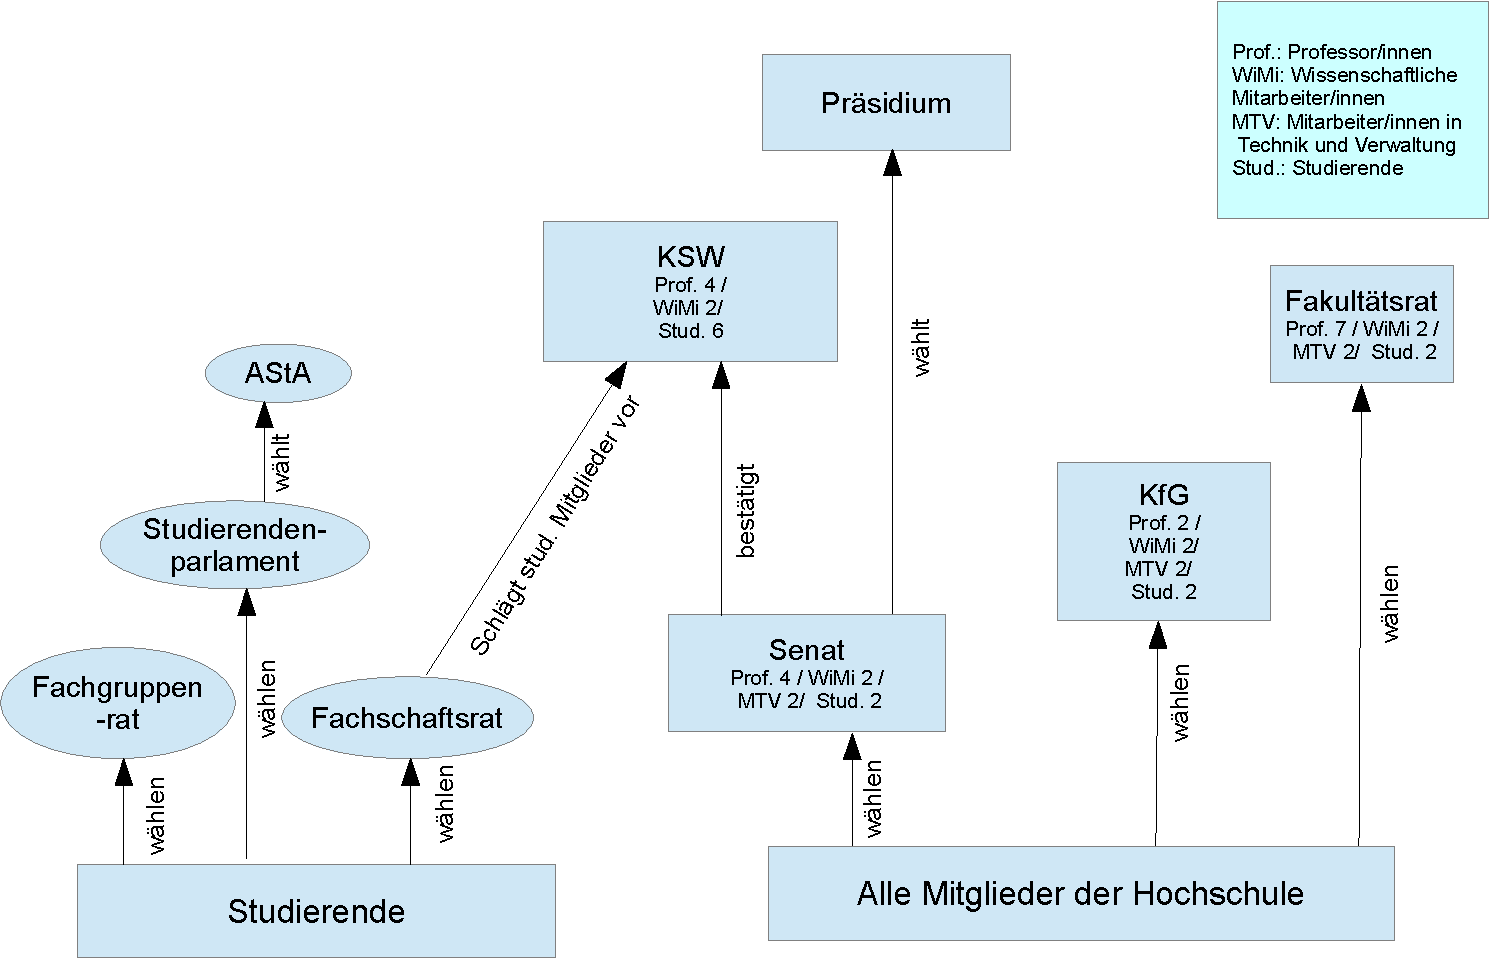
\includegraphics[width=\textwidth]{bilder/gremienkunde/gremienkunde3}
		\end{center}
		\end{minipage}
		\vspace{0.5cm}
		
		\begin{multicols}{2}
		\subsection{Fachgruppe}
\label{fachgruppe}
\url{http://fginfo.cs.tu-bs.de}

Die Fachgruppe seid ihr! Im Grunde besteht die Fachgruppe aus sämtlichen Studierenden der Fachrichtung Informatik. Diese wählen einen Fachgruppenrat der sich dann für die Interessen aller einsetzt. 
Im Fachgruppenraum IZ150 stehen dir jederzeit zuverlässige Mitstudierende zur Verfügung denen du Fragen bezüglich deines Studiums und allem drumherum stellen kannst. Einige davon sind auch Mitglieder des Fachgruppenrats und sind dafür verantwortlich, die Meinungen aller Informatikstudierenden gegenüber der Fakultät und in verschiedenen Kommissionen zu vertreten. Eine richtige Trennung zwischen Fachgruppenrat und Fachgruppe besteht also nicht. Also komm vorbei, bringt dich ein und engagier dich für unsere Studienrichtung. Oder hol dir einfach ein paar koffeinreiche Erfrischungen. 

		\subsection{Hochschulpolitik -- Einmischen an der Universität}

Auch wenn ihr jetzt erst ein Studium aufgenommen habt, habt ihr sicherlich 
schon mitbekommen, dass an der TU nicht immer alles rund läuft.

Was vermutlich nur die Wenigsten wissen: Auch als Studierende kann man sich 
dafür einsetzen, dass sich etwas ändert. So gibt es für nahezu alle Belange Gremien 
an der Uni, wo auch fast immer Studierende mitmachen, oft sogar mit Stimmrecht. 
Obwohl wir Studierenden die größte Gruppe der Uni sind, haben wir dabei aber nahezu immer 
weniger Stimmen als die Professor/innen oder Mitarbeiter/innen. 

Trotzdem lässt sich vieles erreichen. Wer mitmachen möchte, kann einfach 
mal zu einen unserer Fachgruppentreffen kommen. Der aktuelle Termin steht immer 
 auf unserer Webseite \fginfoUrl.

Im folgenden stellen wir euch einmal alle Gremien vor.
Auf der vorherigen Seite findet ihr eine grafische Übersicht über die verschiedenen Gremien. Sie sind dort hierarchisch geordnet.

\subsubsection*{Organe der Studierendenschaft}

Die Studierendenschaft besteht aus allen Studierenden der TU Braunschweig, also auch dir!
Man wird mit der Einschreibung automatisch Mitglied. Dazu gehört auch ein Semesterbeitrag, den jede/r 
zusätzlich zu den Studiengebühren zahlt und womit die Studierendenschaft ihre Aufgaben finanziert. 
Dazu gehören neben dem Semesterticket, dem Hilfsfond für Studierende in Not und der 
Fahrradwerkstatt vor allem die Aufgaben der Fachgruppen, Fachschaften und des AStA. Auch diese
Erstizeitung wurde darüber finanziert.
\\
\\
Die Studierendenschaft gliedert sich wiederum in Fachschaften und Fachgruppen.
Alle Studierenden einer Fakultät bilden zusammen die \textbf{Fachschaft (FS)}, davon gibt es derzeit insgesamt sechs.
Diese werden wiederum in  \textbf{Fachgruppen (FG)} aufgeteilt. Alle Studierenden eines Studienfaches bilden eine Fachgruppe, 
somit besteht die Fachschaft unserer Fakultät aus den Fachgruppen Informatik, Mathematik, Medienwissenschaften, Sozialwissenschaften sowie 
Wirtschaftsinformatik. Die Studierenden einer Fachschaft werden  durch den 
\textbf{Fachschaftsrat (FSR)} vertreten. Da wir viele verschiedene Fächer haben, wichtige Dinge aber oft gemeinsam besprochen werden müssen,
trifft sich bei uns der Fachschaftsrat üblicherweise einmal pro Monat. 
Bei wichtigen Dingen (üblicherweise wenn unerwartet ein bestimmtes Gremium einberufen wird) kann dies auch öfters passieren.
\\
\\
Die meiste und wichtigste Arbeit passiert aber in den \textbf{Fachgruppenräten (FGR)}, 
für die Informatik also im Fachgruppenrat Informatik. Er k"ummert sich um die Belange der
Fachgruppe, beruft die Fachgruppen-Vollversammlungen ein, streitet sich mit der
Fakult"at, wenn es mal wieder Meinungsverschiedenheiten wegen irgendwelcher 
Neuerungen gibt, organisiert die Orientierungseinheit f"ur die Erstsemester, stellt Pr"ufungsprotokolle 
zur Verfügung, informiert 
"uber seinen Blog \fginfoUrl
 und tr"agt das ganze Semester "uber 
Informationen aus den verschiedenen Gremien zusammen, und an euch weiter.
Dazu kommen noch kleinere Veranstaltungen (Spiele-,Grill- und Glühweinabende).
F"ur dich ist der FGR der wichtigste Ansprechpartner, denn auch wenn wir deine Probleme mal nicht l"osen 
k"onnen, dann k"onnen wir dir wenigstens sagen, an wen oder was du dich wenden 
kannst. Damit auch zwischen den verschiedenen Fachschaften
und Fachgruppen kommuniziert wird, 
gibt es das \textbf{Fachschaftenplenum}, was kein Gremium im eigentlichen Sinne 
ist, aber ein Forum zum Meinungs- und Interessenaustausch darstellt. Es trifft 
sich etwa einmal im Monat und ist f"ur jeden offen, der einen Einstieg in die 
Unipolitik sucht. Außerdem nutzen die studentischen Gremienvertreter das Plenum gerne 
um ein Meinungsbild der Fachgruppen und Fachschaften zu aktuellen Entscheidungen einzuholen.

Ganz basisdemokratisch ist auf allen Hierarchie\-ebenen der Studierendenschaft
die jeweilige \textbf{Vollversammlung (VV)} das oberste Organ, allerdings nur
mit empfehlendem Character. Sie findet ein- bis zweimal pro Jahr statt und
dort wird "uber Aktuelles und Wichtiges informiert und/oder abgestimmt. Eine
Vollversammlung aller Studierenden wird vom StuPa-Pr"asidium, eine 
Fachschafts- oder Fachgruppen-VV vom FSR oder FGR einberufen und geleitet.

Womit wir bei Abk"urzungen w"aren, die noch nicht erkl"art wurden: Das \textbf{Studierendenparlament (StuPa, SP)} ist die 
unmittelbare Vertretung aller Studierenden, wird von der Studierendenschaft 
direkt in jedem Semester gew"ahlt und tagt \textbf{hochschul"offentlich}.
Jede/r Studierende hat dort Rede und Antragsrecht, abstimmen können allerdings nur 
gewählten Mitglieder. Sie beschlie"sen studentische Angelegenheiten, verabschieden den studentischen 
Haushalt und w"ahlen den \textbf{Allgemeinen Studentischen Ausschuss (AStA)},
den \textbf{"Ubergeordneten Wahlausschuss ("UgWA)}
und verschiedene weitere Aussch"usse. Das StuPa w"ahlt au"serdem sein eigenes
Pr"asidium, welches die Sitzungen und (uniweiten) Vollversammlungen leitet und
das StuPa nach außen  vertritt.  

Insgesamt ist das StuPa eine der wichtigsten Gremien: Es wählt den AStA, entscheidet über die Verwendung der von den Studierenden bezahlten Semesterbeiträge 
und beschließt nicht zuletzt die endgültige Form des Semestertickets. 
Da die Sitzungen öffentlich ist, kann und sollte jede/r Interessierte sich das mal angegucken.

Von allen studentischen Aussch"ussen ist der \textbf{AStA}  der
Sichtbarste. Er ist das ausf"uhrende Organ der 
Studierendenschaft und vertritt alle Studierenden nach au"sen, z.B. bei 
Verhandlungen mit der BVAG wegen des Semestertickets aber auch gegenüber der 
Landesregierung, sowie nach innen, etwa gegenüber dem Präsidium. Seine Aufgaben werden vom 
StuPa festgelegt und beinhalten neben Serviceangeboten (Fahrradwerkstatt, Kopieren, Binden, 
Internationaler Studiausweis), Beratung (z.B. Sozial- und Rechtsberatung) auch hochschulpolitische 
(z.B. zur Bologna-Reform) und politische (z.B. Wohnungsnot zu Semesterbeginn) Arbeit zu den 
unterschiedlichsten Themen. Zu seiner Unterstützung kann er Referent/innen 
bestellen, die sich hauptsächlich um ein spezielles Aufgabengebiet kümmern.
Der AStA muss sich dem StuPa gegenüber für seine Arbeit verantworten.

Das zweite vom StuPa gew"ahlte Gremium ist der \textbf{"Ubergeordnete 
Wahlausschuss ("UgWA)}, der die studentischen Wahlen organisiert und "uberwacht.

\subsubsection*{Kollegialorgane}

Neben den bis jetzt vorgestellten Organen der Verfassten Studierendenschaft 
gibt es nat"urlich auch noch Schnittstellen zwischen den Studierenden und den anderen 
an der Universit"at vertretenen Personengruppen, den MTV (Mitarbeiter/innen 
aus Technik und Verwaltung), den WiMis (Wissenschaftliche Mitarbeiter/innen) und nat"urlich den Lehrenden (Professor/innen). Hier ist das 
oberste Organ innerhalb der Fakult"aten der \textbf{Fakult"atsrat (FKR)}, 
dem 7 Professor/innen, 2 Studis, 2 MTVler und 2 WiMis angeh"oren. Hier wird all das 
entschieden, was andere Gremien oder das Dekanat erarbeitet haben, bspw. 
"Anderungen an den Prüfungsordnungen. Wird eine Entscheidung getroffen, so gilt diese offiziell und kann umgesetzt werden. Da auf Grund der 
Stimmenverteilung (s.o.) die Professor/innen immer eine Mehrheit haben, m"ussen wir 
in den Gremien, die vorher die inhaltliche Arbeit leisten, versuchen unsere 
und eure Vorstellungen einzubringen. Die studentischen 
Vertreter/innen werden einmal im Jahr, jeweils im Wintersemester, direkt gew"ahlt. Da 
wie gesagt die Studiengänge unserer Fakultät doch durchaus unterschiedliche 
Studieng"ange sind, gibt es einen nicht formellen "`kleinen Fakult"atsrat"', 
die \textbf{Informatik-Kommission}. Die Informatik-Kommission, der drei Professor/innen, 
sowie je ein WiMi, ein MTVler und ein Studi angehören, berät informatikspezifische Dinge und 
bereitet sie für den Fakult"atsrat vor, damit die Entscheidungen im FKR 
schneller gef"allt werden können und sich die Vertreter/innen der anderen Studiengänge nicht so langweilen 
;-).

Das formal oberste Gremium der Uni ist der \textbf{Senat}, der sich mit 
allgemeinen Themen befasst, die "uber der Zust"andigkeit der Fakult"aten 
liegen (als wichtiger Punkt ist hier die Verteilung des universit"aren 
Haushaltes zu nennen). Wie in den FKR ist hier die Stimmengewichtung 7 : 2 : 2 
: 2, auch seine Mitglieder werden j"ahrlich gew"ahlt. Wie das StuPa hat auch der 
Senat die M"oglichkeit für seine Arbeit unterst"utzende Kommissionen einzusetzen.

\subsubsection*{Kommissionen und Aussch"usse}

Da wir so oft Kommissionen und Aussch"usse erw"ahnt haben, seien die drei 
wichtigsten hier kurz vorgestellt: zun"achst ist da die 
\textbf{Studienkommission (StuKo)} zu erw"ahnen.

Sie ist das einzige gemischte Gremium, in dem die Studierenden die Mehrheit 
haben: Neben zwei studentischen Mitgliedern sind außerdem noch ein/e Professor/in sowie ein WiMi stimmberechtigtes Mitglied. 
Dazu kommt ein/e Mitarbeiterin aus Technik und Verwaltung als beratendes Mitglied.
Die Studienkommission erarbeitet vor allem Vorschl"age f"ur die Verbesserung der 
Qualit"at in der Lehre, so werden z.B. Vorschl"age zur "Anderung der 
Studienordnung und der BPO diskutiert. Die Studienkommission muss vor allen 
Entscheidungen des Fakult"atsrates, welche die Lehre, das Studium oder 
Pr"ufungen betreffen, angeh"ort werden. Eingesetzt wird die StuKo von den 
Fakult"atsr"aten, die studentischen Vertreter/innen rekrutieren sich meist aus den 
FSR/FGRn oder deren Umfeld (obwohl theoretisch jede/r Interessierte mitarbeiten 
kann). Die Sitzungen sind hochschul"offentlich, d.h. auch nicht gew"ahlte 
Studierende k"onnen (und sollten) dort jederzeit ihre Stimme einbringen.

%\begin{figure}[h]
%  \centering
\includegraphics[width = 0.7\linewidth]{bilder/comics/otto1_3.png}
%\end{figure}
Auch Professor/innen ist es einmal verg"onnt, sich in den Ruhestand zu begeben oder 
andere Hochschulluft zu schnuppern. Wenn dies ansteht, dann muss die 
freigewordene Stelle (logischerweise) in den meisten F"allen neu besetzt 
werden. Daf"ur wird eine \textbf{Berufungskommission} vom Senat eingesetzt, um 
die Nachfolge zu regeln. Hier werden die Kandidierenden, nachdem eine Vorauswahl 
getroffen wurde, sozusagen auf Herz und Nieren "uberpr"uft, und zwar im Rahmen 
eines "offentlichen Vortrags, den sich jede/r Interessierte anh"oren kann. Die 
 studentischen Vertreter/innen in der Kommission interessiert dabei vor allem, ob 
der/die Kandidat/in f"ahig ist, eine Vorlesung verst"andlich und klar 
strukturiert zu halten oder ob er sich in schweren wissenschaftlichen 
Formulierungen verliert, denn es gibt immer wieder Personen, die sich
haupts"achlich auf die Forschungs- und kaum auf die Lehraufgaben konzentrieren.
Die Berufungskommission 
erstellt nach ausgiebigen Beratungen eine Liste, die, nachdem sie den Fakultätsrat und Senat 
passiert hat, ans ,,Ministerium f"ur 
Wissenschaft und Kultur'' (MWK) weitergeleitet wird, das dann nach dieser 
Liste entscheidet, mit wem es, vertreten durch den Uni-Pr"asidenten, der ja 
formal auch Angestellter des MWK ist, in Verhandlungen tritt.

Ein ziemlich wichtiger, von den FKR eingesetzter Ausschuss ist der 
\textbf{Pr"ufungsausschuss (PA)}. Er besteht aus 5 Mitgliedern (3 Prof. : 1 WiMi : 0 MTV : 
1 Stud. ) und ist f"ur alle Fragen zust"andig, die im Zusammenhang mit Pr"ufungen
auftreten k"onnen. Bei (fast) allen Problemen, die mit Pr"ufungen 
zusammenh"angen, kann
man sich an den Pr"ufungsausschuss wenden -- so k"onnen z.B. weitere
Nebenf"acher auf Antrag der Studierenden vom Pr"ufungsausschuss genehmigt
werden.

Dann gibt es noch die \textbf{Kommission für Studium und Weiterbildung (KSW)}. 
Sie bildet das Gegenstück zur Studienkommission auf zentraler Ebene und arbeitet den Senat sowie dem 
Präsidium zu. Es gibt insgesamt sechs studentische Mitglieder, dazu kommen vier Professor/innen und zwei WiMis. 
Ähnlich wie die StuKo werden hier allgemeine Fragen der Lehre behandelt.

Und -- last but not least -- sei die \textbf{Kommission für Gleichstellung} 
erw"ahnt, das einzige Gremium mit Stimmengleichheit (2 : 2 : 2 : 2). Sie wird von allen 
weiblichen Studentinnen und Mitarbeiterinnen gew"ahlt und bestimmt 
 die universit"are Frauenbeauftragte, die sich f"ur Gleichstellung und 
-berechtigung der Frauen an der Uni einsetzt. Sie "uberwacht beispielsweise, ob 
in den einzelnen Aussch"ussen auch Frauen vertreten sind, ob Frauen in 
irgendeiner Art und Weise diskriminiert werden oder ob die gesetzlichen 
Frauenquoten in den "Amtern eingehalten werden. 

Daneben gibt es nat"urlich noch ungez"ahlte weitere kleine und gro"se Gremien, 
Aussch"usse, Kommissionen und damit verbunden viele viele P"ostchen, die immer 
wieder zu vergeben sind. Wenn ihr also Blut geleckt habt und nicht nur durch 
eure Beteiligung bei den Wahlen Einfluss auf die Hochschulpolitik nehmen wollt, 
dann meldet euch doch im Fachgruppenrat und arbeitet mit -- ihr seid herzlich 
willkommen!

\emph{Quellen: Fachschaftsrat Maschinenbau, FGR Informatik\\WS, PK}

		\end{multicols}
	\newpage

	\section{Sonstiges}
		\label{sonstiges}
		\begin{center}
		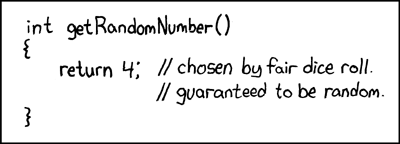
\includegraphics[totalheight=3cm]{bilder/XKCD/random_number}
		\end{center}
		\begin{multicols}{2}
		%\subsection{Studentische Vereinigungen an der Technischen Universität
Braunschweig}
\label{vereinigungen}
%xp
%	\url{http://fginfo.cs.tu-bs.de}
	An der TU Braunschweig gibt es eine Vielzahl studentischer
	Vereinigungen, bei denen ihr euch neben dem Studium einbringen
	könnt. Dabei ist eigentlich für jeden etwas dabei. Die
	vollständige Liste findet ihr unter 
	\url{http://www.tu-braunschweig.de/abt11/studentischevereinigungen/studverein}. 
	Im Folgenden stellen wir einige unserer Ansicht nach für
	Informatik-Studierende besonders Interessante vor.

	\subsubsection{Gesellschaft für Informatik- Studierendengruppe
	Braunschweig}	
	Die Gesellschaft für Informatik e.V. (GI) ist die größte
	Vereinigung von Informatikerinnen und Informatikern im
	deutschsprachigen Raum. Sie versteht sich als Plattform für
	Informatikfachleute aus Wissenschaft und Wirtschaft, Lehre und
	Öffentlicher Verwaltung und versammelt eine geballte
	Konzentration an Wissen, Innovation und Visionen. \\\\
	 Die SG Braunschweig ist gerade noch mitten im Gründungsprozess
	 und somit die jüngste der derzeit 12 SGen in Deutschland. Die
	 SGen repräsentieren an Informatik interessierte junge Menschen,
	 ohne dabei begrenzt zu sein auf einen einzelnen Studiengang
	 oder eine einzelne Hochschule, und sorgen durch ihre Vernetzung
	 untereinander auch für den überregionalen Austausch. Dazu
	 wollen wir Veranstaltungen organisieren. 

\subsubsection{Wissenschaftliche Arbeitsgemeinschaft für Studio- und Senderfragen an der TU Braunschweig}
Die ags gibt Studierenden die Gelegenheit während ihres Studiums
praktische Erfahrungen in der Fernseh- und Medientechnik, sowie in
allgemeiner Elektronik zu sammeln. 


Neben den zahlreichen externen Produktionen, z.
B. den Vorlesungen der Kinder-Uni und des MacGyver-Ideenwettbewerbs, die
von der ags begleitet werden, betreibt sie in ihren Räumen 
ein professionelles Fernsehstudio. 
\\\\
 Im Elektroniklabor ,,e.lab'' finden sich sich sechs
 vollausgestattete Elektronikarbeitsplätze, die von jedem Studierenden
 genutzt werden können. Darüber hinaus gibt es ein umfangreiches
 Kursangebot an, z.B. die begehrten Mikrocontrollerkurse. 
\\\\
  Organisiert von Studierenden als gemeinnütziger Verein ist die ags
  seit 1953 für Studierende aktiv. 
  \\\\
   Sie trifft sich jeden Dienstags und Donnerstags ab 19:00 Uhr in der
   Zimmerstraße 24c, ,,Keller des Grotrian''. Komm einfach vorbei!


		% !TEX root = ../../1-te.tex

\subsection{Ansprechpartner}

	\paragraph{Fachgruppenrat}
		Im Normalfall treffen wir uns jede Woche zum Fachgruppentreffen im Raum 149/150 des Informatikzentrums. Den  Termin findest du auf unserem Blog \fginfoUrl. Falls du eine Frage hast, kannst du gerne zum regulären Fachgruppentreffen kommen, oder einfach so mal vorbei schauen, ob jemand da ist. Gerade im Semester sind die Chancen gut, einen von uns anzutreffen ;)
		\\
		\\
		Tipp: In der Stunde vor dem Treffen füllt sich der Raum schon langsam, also hast du da gute Chancen, Probleme in kleinerer Runde zu besprechen. Ansonsten erreichst du uns natürlich via Email unter \verHref{6}{mailto:fginfo@tu-bs.de}{fginfo@tu-bs.de}. 

	\paragraph{Fachspezifisches}
		Bei Fragen zu einem speziellen Fach wendest du dich am
		besten an den oder die Professor/in bzw. Dozent/in -
		keine/r von denen beißt! Am besten findest du sie über die Seiten der jeweiligen Institute 
		oder über die Personensuche unter \verUrl{6}{http://www.tu-braunschweig.de/suchoptionen/personen}.

	\paragraph{Studiengangskoordinatorin}
		Yvonne Sehnert \\
		Sie steht bereit, um deine Fragen zu beantworten, und für alles, was sie nicht selbst weiß, weiß sie, an wen sie die Frage weiterleiten muss.\\
		Carl-Friedrich-Gauß-Fakultät\\
		Rebenring 58 A | Raum 124\\
		Sprechzeiten: Nach  Vereinbarung\\
		Telefon: (0531) 391-2843\\
		E-Mail: \verHref{6}{mailto:informatik-studium@tu-bs.de}{informatik-studium@tu-bs.de}

	\paragraph{Prüfungsamt}
		Rebecca Weidner\\
		Carl-Friedrich-Gauß-Fakultät\\
		Rebenring 58 A | Raum 127\\
		Tel.: (0531) 391-2844\\
		Fax: (0531) 391-8220\\
		E-Mail: \verHref{6}{mailto:pa-informatik@tu-braunschweig.de}{pa-informatik@tu-braunschweig.de}\\
		Sprechzeit im Semester:\\
		Di. und Do.: 10:00–12:00 Uhr und 14:00-16:00 Uhr\\
		Sprechzeit in der vorlesungsfreien Zeit:\\
		Di. und Do. 10:00-12:00 Uhr

		% !TEX root = ../../1-te.tex

\subsection{Campuskarten und Raumnummern}
\label{campuskarte}
Eine aktuelle Campuskarte, die durchsucht werden kann, findet sich unter \verUrl{2}{http://tinyurl.com/tubsmap}.

Ein Raumplan für das 1. und 2. OG des Informatikzentrums findet sich
unter \verUrl{2}{http://www.ibr.cs.tu-bs.de/rooms/rooms.html}

%Sollten euch die genannten Links zu unhandlich zum Abtippen sein, findet ihr
%auch alle auf unserem Blog. Dort findet ihr auch virtuelle Campustouren, die  in einem Web 2.0 Seminar entstanden und
%%bei Google Maps gehostet sind.

Für die Suche nach einem Raum solltet ihr noch wissen, wie sich die Raumnummern bilden: Bei Nummern wie \textit{PK 15.1} sind die Buchstaben ein Kürzel für die Straße, in dem das Gebäude liegt. Die Zahl vor dem Punkt ist meist die Hausnummer, und nach dem Punkt eine willkürliche Durchnummerierung. Anders bei Kürzeln wie \textit{IZ 150}, bei denen IZ das Informatikzentrum an der Mühlenpfordstraße meint, die erste Stelle für die Etage steht und bei beiden letzten den Raum innerhalb der Etage. Die \textit{Plaza} ist der große Platz im ersten Stock bei den Aufzügen.

		\end{multicols}
		\newpage
		\subsection{Lernräume}
	Hier wollen wir euch eine aktuelle Übersicht über Lernräume an der TU Braunschweig geben. Die Liste ist im Moment nicht vollständig. Auf unserem Blog pflegen wir eine Liste, die wir immer dann erweitern, wenn wir einen neuen Lernraum finden.
Wenn du im Laufe deines Studiums einen guten Ort findest, kannst du uns den Raum mitteilen, wir überprüfen das und nehmen ihn dann in die Liste auf.. Alle Gebäude stehen, wenn nicht anders in Anlage 1 der Hausordnung der TU Braunschweig erwähnt, von 7:30 bis 19:30 Uhr offen.
	\subsubsection*{Informatikzentrum}
		\begin{tabular}{|p{4cm}|p{5cm}|p{8cm}|}
			\hline Raum & Öffnungszeiten & Ausstattung \\ 
			\hline Plaza des Informatikzentrums & normal &  Tische und Stühle, Steckdosen unter Bodenabdeckungen zu finden \\
			\hline Fachgruppenraum der Informatik IZ 150 &
			nach Absprache mit Mitgliedern des
			Fachgruppenrates (wir ;) ) & Kaffemaschine,
			Sofas, Tische, WLAN, Steckdosen in Massen sowie Ethernetkabel\\ 
			\hline Fachgruppenraum der Wirtschaftsinformatik
			IZ 159 & nach Absprache mit Mitgliedern des
			Fachgruppenrates Wirtschaftsinformatik & Sofas, Tische, WLAN und Steckdosen \\ 
			\hline CIP Pool IZ G40 & normal & Rechner-Pool mit Linux-PCs, Tafel\\ 
			\hline Gruppenarbeitsraum IZ 033 & 
			
			Solange nicht anders belegt. Den Schlüssel
			erhält man gegen Pfand im Seketariat der Robotik bei Frau Engel,
			Raum G13.
			 &
			Tische, Stühle, WLAN
			\\
			\hline
		\end{tabular}
	\subsubsection*{Andere Lernräume}
		\begin{tabular}{|p{4cm}|p{5cm}|p{3.6cm}|p{4cm}|}
 			\hline Raum & Öffnungszeiten & Ausstattung & Anmerkung  \\  
			\hline Grotrian  Zimmerstraße 24 & Normal  &
			Alte Tische und Stühle, WLAN, vereinzelt Tafeln & Wenn Mitglieder der verschiedenen Fachgruppen anwesend sind hat das Grotrian meist länger offen. Da dies oft der Fall ist kann man hier meist lange lernen. \\ 
			\hline Bibliothek & Mo - Fr: 07:00 - 24:00 Sa:
			10:00 - 20:00& Niedrige Tische und Stühle,
			Ruhezone, WLAN, Rechnerarbeits\-plätze, Kopierer &  nicht zum  Lernen in der Gruppe  geeignet \\ 
			\hline Mensa / Cafeteria & Mo -Do: 08 - 20:00 Uhr Fr: 08:00 - 15:00 & Tische, Stühle, kein (!) WLAN, einzelner Rechner mit Netzzugang, Verpflegung incl. Selbstbedienungs-Kaffeeautomat& Probleme: Nicht durchgehend geöffnet, die Plätze sind primär zu Essen gedacht, von Lernsessions zu den Stoßzeiten sollte man also im eigenen und fremden Interesse absehen. \\ 
			\hline Bei dir zuhause & immer & Deine Sache & Achtung: Ablenkung ;) \\ 
			\hline Das eine oder andere Cafe / Kneipe & kommt drauf an & wechselhaft &Siehe die beiden vorherigen \\
			\hline
		\end{tabular}

		\newpage
		% !TEX root = ../1-te.tex

\begin{description}
\item[Herausgeber:]
	Fachgruppe Informatik\\
	c/o AStA der TU Braunschweig\\
	Katharinenstraße 1\\
	38106 Braunschweig\\
	Tel.: 0531/391-4569\\
	E-Mail: \verHref{5}{mailto:fginfo@tu-bs.de}{fginfo@tu-bs.de}\\
	Webseite: \fginfoUrl
\tocheck{4}{Mitglieder das FG-Rats nennen}
\item[Cover:] Sophia Scholtka und Rebecca Finster
\item[Comics:] Randall Munroe -- XKCD (\verUrl{5}{http://xkcd.com/})
\end{description}

\end{document}
